\section{Introduction}
This section will provide the theoretical background necessary to motivate and understand the context of rest of the thesis.
It starts with an brief overview of successful works done by the Standard Model (SM) in the particle physics, and review the remained homework (widely referred from \cite{Peskin} and \cite{QandL}).
The concept of supers-symmetry is then introduced as potential yet strong candidate of the solution by extending the SM.
A particular emphasis is put on the Minimal Super-Symmtric Standard Model (MSSM), with closely outlining the phenomenology and present experimental constraints.
Finally, the experimental signature targeted in the thesis is explained as well as discussing the searching strategy. \\


\subsection{The Standard Model of Elementary Particles}
The particle content of the SM is shown in Tab. \ref{tab::Introduction::SMFermions} and Tab. \ref{tab::Introduction::SMBosons}. There are three types of particles: fermions with the spin of 1/2 that consists matters: gauge bosons with the spin of 1 mediating the interaction acting between particles: and the spin-0 Higgs boson feeding their masses through the the Brout-Englert-Higgs (or BEH) mechanism. \\

\tab{c | c c c | c c c c c}
{
\hline
        &  \multicolumn{3}{c|}{Generation} &   $Q$ &  $T$  & $T^3$ &  $Y$ & $N_C$\\
\cline{2-4} 
        &  1st   &  2nd    &  3rd         &     &     &    &   \\
\hline
\hline
Quarks  &  $\colv{u \\ d}_{\mL}$   &  $\colv{c \\ s}_{\mL}$    &  $\colv{t \\ b}_{\mL}$ &   $\colv{2/3 \\ -1/3}$ &  1/2  & $\colv{1/2 \\ -1/2}$ &  $1/3$ & 3\\
        &  $u_{\mR}$   &  $c_{\mR}$    &  $t_{\mR}$ &   $2/3$  &  0  & 0 &  $4/3$  & 3\\
        &  $d_{\mR}$   &  $s_{\mR}$    &  $b_{\mR}$ &   $-1/3$ &  0  & 0 &  $-2/3$ & 3\\
\hline
Leptons  &  $\colv{\nu_e \\ e^-}_{\mL}$   &  $\colv{\nu_\mu \\ \mu^-}_{\mL}$    &  $\colv{\nu_\tau \\ \tau^-}_{\mL}$ &   $\colv{0 \\ -1}$ &  1/2  & $\colv{1/2 \\ -1/2}$ &  $-1$ & 0 \\
        &  $e_{\mR}$   &  $\mu_{\mR}$    &  $\tau_{\mR}$ &   $-1$  &  0  & 0 &  $-2$ & 0 \\
\hline
}
{Fermion contents in the SM. The quantum numbers $Q$, $T$, $T^3$ and $Y$ are respectively electroc charge, weak isospin number, the third component of weak isospin and weak hyper charge. $N_C$ represents the number of color states. The subscripts L, R indicate the chirality (left- or right-handed respectively), and the pharenthses denote the $SU(2)_L$ doublet.
}
{tab::Introduction::SMFermions}


\tab{c c | c c c c c}
{
\hline
             &          &  $Q$ &  $T$  & $T^3$ &  $Y$ & $N_C$ \\
\hline
\hline
gluon        & $g$      &   0  &  0    &  0    &  0   &  8    \\
\hline
weak bosons  & $W^\pm$  &$\pm1$&  1    &$\pm1$ &  0   &  0    \\
             & $Z$      &   0  &  0    &  0    &  0   &  0    \\
\hline
photon       & $\gamma$ &   0  &  0    &  0    &  0   &  0    \\
\hline
\hline
higgs       & $h$       &   0  &  1/2  &  -1/2 &  1   &  0    \\
\hline
}
{Gauge bosons and higgs in the SM. The notation for the quantum numbers are the same with \ref{tab::Introduction::SMFermions}.}
{tab::Introduction::SMBosons}


The three types of gauge bosons; gluon ($g$); weak bosons ($W^{\pm},Z$) and photon ($\gamma$) respectively characterize strong interaction, weak interaction and electromagnetic interaction. 
%\footnote{Gravity has yet been accommodated by the SM and any successful extension of it.}
Fermions are further two-hold: quarks which senses all the three interactions: lepton which couple only via weak and eletromagnetic interaction. Both family have up- and down-type, together with two more duplications of them (``2nd / 3rd generation'') with exactly the same properties except the masses. Each fermions furthermore have the charge conjugated partner called anti-fermions. \\


\subsubsection{The Gauge Principle and Particle Interaction} \label{sec::Introduction::gaugePrinciple}
A successful theory for elementary particles must be quantum and relativistic.
The theory of SM is constructed in a relativistic framework of field theory, fully exploiting the virtue that time ($t$) and position ($\bm{x}$) are treated equivalently; both are parameters of coordinates rather than observables. It is characterized by a Lorentz-invariant Lagrangian in which particles are described by a function in terms of $x^\mu$ (``fields'') following the Lorentz transformation law of corresponding spin expression. The free Lagrangian for fermions are given by:
\begin{align}
\mathcal{L} = i \bar{\psi} \gamma_\mu \partial_\mu \psi - m \bar{\psi}\psi + \mathrm{h.c.}
\label{eq::SMfreeLag}
\end{align}
where $\psi$ is spinor field for a fermion with the mass of $m$, and $\gamma_\mu$ is $4\times4$ gamma matrices. \\
The first term corresponds to the kinetic terms and the second is to the mass term.
%\begin{align}
%\colv{\bm{1} & \\ \bm{1} & }
%\mathrm{(In Weyl's representation)}
%\end{align}
%Note that $\sigma_i$ are Pauli's matrices

Interaction between particles are ruled by a local symmetries called ``gauge symmetry''. 
The interaction terms are obtained by requiring the free Larganian for invariance against gauge transformation which is for instance a $U(1)$ transformation in case of electromagnetic interaction:
\begin{align}
\psi \ra e^{i\theta(x) Q} \psi = e^{i\theta(x) q} \psi
\end{align}
where $Q$ is the generator of the $U(1)$ transformation, $q$ is charge that the fermion $f$ has, and $\theta(x)$ is an arbitrary time-space dependent phase.
The free Lagrangian in Eq. (\ref{eq::SMfreeLag}) is not invariant under this transformation, however can be fix by employing a small hack in the differential ($\partial_\mu$) terms in the free Lagrangian:
\begin{align}
\partial_\mu \ra D_\mu := \partial_\mu - ieA_\mu (x)
\end{align}
where $A(x)$ is a vector field transformed by the gauge transformation by:
\begin{align}
A_\mu \ra A_\mu + \frac{1}{e} \partial_\mu \theta(x).
\end{align}
%The replaced $D_\mu$ is referred to ``covariant differential''.

The interaction term emerges as the extra terms in the Lagrangian:
\begin{align}
\mathcal{L}_{\mathrm{int.}} = e\bar{\psi} \gamma^\mu \psi A_\mu.
\label{eq::SMfreeLag}
\end{align}
From the consistency with classical Maxwell equation, this represents the interaction between fermion $f$ and electromagnetic
and $A_\mu$ is identified as the electromagnetic potential in the classical electromanetism or the particle field for photon. \\



\subsubsection{Perturbation and Renormalization}
The effect of interaction is often characterized via transition amplitude from an initial state ($i$) to a final state ($f$):
\begin{align}
\bra{f} e^{-i\mathcal{H}_{\mathrm{int.}}t} \ket{i},
\end{align}
which is a basic quantity for phenomenological prediction on interaction cross-section or decay branch. 
This is however in most of the cases not analytically calculable therefore done through a perturbation expansion based on the coupling constant of the interaction, for which $\alpha := e^2/4\pi$ is conventionally used for electromagnetic interaction. 


While the small coupling constant of electromagnetic interaction $\sim 1/137$ is supposed to guarantee a good convergence behavior of the expansion, as well as to provide validity of calculation with truncated orders in the series, it is however found that the higher order terms immediately lead to divergence quite everywhere in cross-section calculation (infrared / ultraviolet divergences). This problem was solved by a procedure called ``renormalization'' 
%\cite{Tomonaga}\cite{Feynman}, 
where physical parameters (i.e. the masses and coupling constants) are redefined to absorb the infinities, resulting in a finite cross section calculation. Historically, it is firstly formulated successfully in QED, and then understood by that the gauge symmetry played an important role in calceling the divergence \cite{Ward1950}\cite{Takahashi1957}. From this moment, gauge symmetry started establishing the status as a guidance principle in constructing theory, beyond merely a prescription. It is also shown with considerable generality that well-behaving theory (``renormalizable theory'') must respect gauge symmetry \cite{tHooft1972}. \\

Also the concept of renormalization provided a critical insight that the magnitude of physics parameters in a theory could effectively vary depending on the energy scale with which the interaction happen. The evolution is characterized by the renormalization group equation (RGE), for example, as for the coupling constant ($\alpha$): 
\begin{align}
\dfrac{1}{\alpha(Q)^2}-\dfrac{1}{\alpha(Q_0)^2} = -\dfrac{\beta(\alpha)}{2\pi} \log{\left(\dfrac{Q}{Q_0}\right)},
\end{align}
where $Q$ is the scale defined by the typically momentum transfer of interaction processes, and $\beta(\alpha)$ is the beta function, proportional to $\alpha^2$ at 1-loop level. This evolution is known as the ``running'' effect, which is an useful proxy for exploring the behavior of theory over the scale. \\


\subsubsection{QED, QCD, and the Electroweak Theory}
The Lagrangian for Quantum Electromagnetic Theory (QED) is given by adding the kinetic terms for photon $-\frac{1}{4}F_{\mu\nu} F^{\mu\nu}$ to one obtained in Sec. \ref{sec::Introduction::gaugePrinciple}:
\begin{align}
\mathcal{L} = -\frac{1}{4}F_{\mu\nu} F^{\mu\nu} + i \bar{\psi} \gamma_\mu \partial_\mu \psi - m \bar{\psi}\psi \, + \mathrm{h.c.}
\end{align}
with $F_{\mu\nu}$ being the field strength:
\begin{align}
F_{\mu\nu} := \partial_\mu A_\nu - \partial_\nu A_\mu.
\end{align}


Similar to what is done in QED with the gauge group of $U(1)$, the Lagrangian for strong and weak interaction can be generated by considering gauge groups of $SU(2)_L$ and $SU(3)$:
$$
\psi \ra e^{i \theta_a(x) \lambda^a}, \psi \,\,\,\,\,\,\,\, a=1,2,\dots (N^2-1) \,\,\,\,\,\, \mbox{\phantom{MM}  (for $SU(N)$)} 
$$
where $\lambda^a$ are the generators of the gauge group. \\
The choice of gauge groups are respectively motivated by observation of approximately valid iso-spin symmetry in the theory of nucleus decay, and an enhanced number of degree of freedoms by factor about 3 for quarks implied by the measurement in $ee\ra qq$. \\

The Lagrangian for strong interaction is:
\begin{align}
\mathcal{L}_{\mathrm{QCD}} & = -\frac{1}{4} \bm{\hat{G}}_{\mu\nu} \bm{\hat{G}}^{\mu\nu} + \,\, \bar{q}(i \gamma_\mu D_\mu - m) q + \mathrm{h.c.}, \nn \\
D_\mu & := \partial_\mu + ig_s \sum_{a=1}^8 G^a_{\mu}\frac{\lambda_a}{2} \nn \\
\bm{\hat{G}}_{\mu\nu} & := \partial_\mu \bm{G}_\nu - \partial_\nu \bm{G}_\mu - g_s \, \bm{G}_\mu \times \bm{G}_\nu, \nn \\
\bm{G}_\mu & := \{G^a_\mu; a=1,2,\dots,8\}
\label{eq::QCDLag}
\end{align}
where $G^a_\mu$ and $q$ represent the fields for gluons and quarks respectively.
$g_s$ the related to the coupling constant $\alpha_s$ by $\alpha_s = g_s^2/4\pi$. 
The charge of strong interaction is called ``color'' (red, blue, green), and the theoretical framework is referred to Quantum Chromo Dynamics (QCD). 
Quarks are in the triplet and gluons are in the octet expression with 3 and 8 degenerated states respectively.
In addition, due to the non-abelian nature of $SU(3)$, gluon has self-interaction with coupling to itself. 
One distinct characteristic for the strong interaction is the negatively slope of running coupling:
\begin{align}
\alpha_s(Q) = \frac{4\pi\alpha_s(\mu_R)}{4\pi + \beta_0 \alpha_s(\mu_R)\log{(Q^2/\Lambda^2_{\mathrm{QCD}})} }
\end{align}
where $\beta = 11 -2n_f/3$ ($n_f$ is number of quarks with the mass above $Q$), $\mu_R$ the renormalization scale (a reference scale of renormalization, different from the physical energy scale $Q$), and $\Lambda_{\mathrm{QCD}}$ the QCD cut-off scale at $\sim 200\mev$. The indication of $\beta<0$ is decreasing coupling constant with increased energy scale $Q$.
Despite of the generally larger coupling than that of electromagnetic interaction, in the energy scale interested in LHC ($Q>100^gev$), $\alpha_s$ typically about 0.1, which is small enough to recover the perturbative picture (``asymptotic freedom''). 
On the other hand, the coupling becomes increasing strong as approaching to $\Lambda_{\mathrm{QCD}}$ leading to immediate catastrophe of perturbation, forcing colored particles to unite each to form color singlet state (``confinement''). \\


Weak interaction is described by a larger gauge group $SU(2)_L \times U(1)_Y$, in a manner residing the electromagnetic interaction altogether. The basic idea for this is to consider that they share the common origin at high energy scale and branch into separate interactions at some point through a spontaneous symmetry breaking (SSB) $SU(2)_L \times U(1)_Y \ra U(1)_Q$.
The regime of unified interaction is commonly referred as electroweak interaction (EW). \\

The gauge transformation distinguishes chirality of fermions, in that $SU(2)_L$ electively acts on left-handed component, expressing the parity violaing nature of weak interaction:
\begin{align}
& \psi_{\mL} \ra e^{i\theta T+i\Theta Y} \psi_{\mL}   \\
& \psi_{\mR} \ra e^{i\Theta Y} \psi_{\mR}.
\end{align}
The Lagrangiaon arrives at:
\begin{align}
\mathcal{L}_{\mathrm{EW}} & = -\frac{1}{4} \bm{\hat{W}}_{\mu\nu} \bm{\hat{W}}^{\mu\nu}-\frac{1}{4}B_{\mu\nu} B^{\mu\nu} + \,\, \bar{\psi}(i \gamma_\mu D_\mu - m) \psi + \mathrm{h.c.}, \nn \\
%
D_\mu & := \partial_\mu + ig \sum_{a=1}^3 W^a_{\mu} \tau_a  + ig^{'} \frac{Y}{2} B_\mu \nn \\
\bm{\hat{W}}_{\mu\nu} & = \partial_\mu \bm{W}_\nu - \partial_\nu \bm{W}_\mu - g \bm{W}_\mu \times \bm{W}_\nu \nn \\
\bm{W}_\mu & := \{W^a_\mu; a=1,2,3\} \nn \\
B_{\mu\nu} & = \partial_\mu B_\nu - \partial_\nu B_\mu
\label{eq::EWLag1}
\end{align}
where $W^a_\mu$ and $B\_mu$ are the fields of EW gauge bosons, and $g, g^{'}$ are the coupling respectively for $SU(2)_L$ and $U(1)_Y$. $\bm{\tau} (= \bm{\sigma}/2)$ are generators of $SU(2)$. \\

The Lagrangian can be also re-written by introducing currents:
\begin{align}
\mathcal{L}_{\mathrm{EW}} & = -\frac{1}{4} \, \sum_{a-1}^3 W^a_{\mu\nu} W^{a\mu\nu}-\frac{1}{4}B_{\mu\nu} B^{\mu\nu} \nn \\
& -\frac{g}{2} (J_\mu^+ W^{-\mu} + J_\mu^- W^{+\mu}) -g J_\mu^3 W^{3\mu} - \frac{g^{'}}{2}J_\mu^YB^\mu  + \mathrm{h.c.}  \nn \\
 J^{\pm}_\mu & := \frac{1}{\sqrt{2}} (W_\mu^1\mp iW_\mu^2) \nn \\
 J^a_\mu & := \bar{\psi}_L \gamma^\mu \tau_q W_\mu^a \psi_L \nn \\
 J^Y_\mu & := Y \bar{\psi}_L \gamma^\mu  \psi_L.
\label{eq::EWLag2}
\end{align}
$J_\mu^\pm$ represent currents changing $T_3$, while $J_\mu^0$ and $J_\mu^Y$ neutral current conserving either $T_3$ and $Y$. \\

The consequence of EW symmetry breaking is implemented by mixing $(W_\mu^3, B_\mu)$ into $(Z_\mu, A_\mu)$:
\begin{align}
\colv{Z_\mu \\ A_\mu} := 
     \left(
   \begin{array}{cc}
     \cos{\theta_W} &  -\sin{\theta_W} \\ 
     \sin{\theta_W} &  \cos{\theta_W} 
   \end{array}
     \right)
 \colv{W_\mu^3 \\ B_\mu}
\end{align}
with a mixing angle (Weinberg angle $\theta_W$) of:
\begin{align}
\tan{\theta_W} := \frac{g^{'}}{g}.
\end{align}
%
The current terms in the Lagrangian Eq. (\ref{eq::EWLag2}) then becomes:
\begin{align}
 & -\frac{g}{2} (J_\mu^+ W^{-\mu} + J_\mu^- W^{+\mu})  \nn \\
 & + \frac{g}{\cos{\theta_W}} \left( -\cos^2{\theta_W} J_\mu^3 + \frac{\sin^2{\theta_W}}{2} J_\mu^Y  \right) \, Z^{\mu}  \nn \\
 & - g\sin{\theta_W} \left( J_\mu^3 + \frac{1}{2} J_\mu^Y \right) A^\mu  \nn \\
\end{align}
By choosing $Y := 2(Q-T^3)$, $A_\mu$ is associated with the gauge field of electromagnetic interaction, 
and the electric charge is found to be related to the weak coupling constant by the Weinberg angle: $e=g\sin{\theta_W}$.


\subsubsection{Electroweak Symmetry Breaking and the Higgs boson}
One outstanding problem in the EW Lagrangian is the prohibition of mass terms, for both gauge bosons and fermions, since they explicitly violates the gauge invariance. 
%since left-handed and right-handed fields obey different $SU(2)_L$ gauge transformation:
%\begin{align}
%  m\bar{\psi}\psi = m \bar{\psi}_{\mL} \psi_{\mR}.
%\end{align}
The BEH mechanism is then employed to solve the problem, where assuming a $SU(2)$ doublet $\phi$ ($Y=-1, T=1/2$) with scalar fields $\phi=(\phi_1,\phi_2)=(\phi^+,\phi^0)$,  and a potential $V(\phi)$ added in the Lagrangian:
\begin{align}
\mathcal{L}_{\mathrm{Higgs}} & := \left(D_\mu \phi \right)^\dg \left(D^\mu \phi \right) - V(\phi) \nn \\
                     V(\phi) & := \mu^2 \phi^\dg \phi + \lambda (\phi^\dg \phi)^2.
\label{eq::HiggsPotential}
\end{align}
While the minimum of the potential is always found in $\phi=(0,0)$ in the $\phi_1-\phi_2$ plane when $\mu^2>0$, 
negative $\mu^2$ leads to non-trivial minima in $v := |\phi|^2 = -\mu^2/2\lambda$ causing the shift of the vacuum expectation value : $<\phi>=0 \ra v$ (spontaneous symmetry breaking). \\

Retaining the origin of $\phi$ as:
\begin{align}
\phi = \colv{0 \\ v+h(x)}
\label{eq::SSB}
\end{align}
and applying the $\partial\mu \ra D\mu$ prescription to Eq. (\ref{eq::HiggsPotential}),
one finds the mass terms for $W,Z$ as:
\begin{align}
m_W & = gv/2 \nn \\
m_Z & = \sqrt{g^2+g^{' 2}} v/2, \nn
\end{align}
where the mass for $W$ and $Z$ is successfully provided.\\

The mass for scalar field $h$ is also found to be:
\begin{align}
m_h & = \sqrt{-2\mu^2}.  \nn
\end{align}
thus $h$ can be also regarded is physical mode, referred as higgs particle. \\

The fermion masses are fed by adding extra terms into Lagrangian:
\begin{align}
\mathcal{L}_\mathrm{Yukawa} := -\bar{\psi}_{i,L} y^{a}_{ij} \phi_a \psi_{j,R} -\bar{\psi}_{i,R} y^{a}_{ij} \phi^\dg_a \psi_{j,L} \nn 
\end{align}
where $i, j=1, 2, 3$ index the generations of fermions, and $a$ denote type of fermions (``up-type quarks'',``down-type quarks'',``leptons'') and $\phi_a$ corresponds to $\phi, \phi^{c}, \phi$ respectively. $y^a_{ij}$ are Yukawa matrices, $3\times 3$ matrices spanned over the family space.
The off-diagonal components in $y^a_{ij}$ are responsible for mixing between generation, which are all zero for leptons, while they are non-zero and the Yukawa matrices are diagonalized by CKM matrix in case of quarks. \\

Inserting Eq. (\ref{eq::SSB}), $\mathcal{L}_{\mathrm{Yukawa}}$ is finally reduced to:
\begin{align}
\mathcal{L}_{\mathrm{Yukawa}} & = \sum_f y_f v \bar{\psi} \psi + y_f \bar{\psi}{\psi} h \nn \\
& = \sum_f m_f \bar{\psi} \psi + y_f \bar{\psi}{\psi} h,
\end{align}
where $f$ is the index of fermions and $y_f$ is the eigenvalues of corresponding Yukawa matrix. \\


Higgs boson (Breit-Englere-Higgs boson) was discovered in LHC in 2012, bringing the last piece of the Standard Model in human knowledge. Measurements on its properties including the mass, spin and coulplings follow, and they show all consistent to the SM at the moment. Precision measurement on its couplings is planning in the later stages in LHC.
%\begin{align}
%\end{align}


%\subsubsection{Standard model processes in LHC}

%\subsubsection{Summary of the SM Lagrangian}
%The complete list of the SM Lagrangian is given by:
%\begin{align}
%\mathcal{L}_{\mathrm{SM}}
% & = -\frac{1}{4} F_{\mu\nu} F^{\mu\nu} \\
% & = i \bar{\psi}\gamma_{\mu}D^\mu \psi + \mathrm{h.c.} \\
% & = \psi_i y_{ij} \psi_j + \mathrm{h.c.} \\
% & = |D_\mu \phi|^2 - V(\phi).
%\end{align}




%
%
\clearpage
\subsection{Remained problems for the Standard Model}
There a couple homework from the SM, from critical ones to potential issues.
A overview is provided in this sub-section, with a focus on problems in which SUSY is particularly motivated as the solution.


\subsubsection{Quadratic Divergence of Higgs Mass}
While the divergences that appears in higher order calculation in SM are universaly cured by renomrlization, the only exception is the mass of higgs boson \ref{fineTune_Barbieri1987}. Since the SM higgs has no parter that is in the same multiplet represented by a certain symmetry, there is no counter terms possible to cancel the leading quadratic divergence happening in the self-energy correction, forcing the higgs mass to explicitly contain the dependence on the cut-off scale $\Lambda$ upto which the loop momentum is integrated.
For instance, the loop correction given by a top-quarks loop is:
\begin{align}
\Delta m_h ^2 = - \frac{3|\lambda|^2}{8\pi^2} \Lambda^2 + O\,(\log\Lambda). 
\label{eq::naturalness1}
\end{align}
%
\begin{align}
m^2_{h,\mathrm{obs.}} = m^2_{h,\mathrm{bare}} + \Delta m_h ^2
\label{eq::naturalnessBare}
\end{align}
%The magnitude can be order of $10^{38} \gev^2$ when assuming SM is valid upto Planck scale: $\Lambda \sim 10^19$, or $10^{8} \gev^2$ with the more pessimistic scnario where SM is only valid upto around scale that has been experimentally explored: $\Lambda \sim 10\tev$. Given the experimental mass is $125\gev$, a naive conclusion is that the tree-level higgs mass $m_h^{\mathrm{bare}}$ and total radiative correction $\Delta_h$ has to cancel in a precision of $10^{-38 \sim -8}$.
The magnitude can be order of $10^{38}$ when assuming SM is valid upto Planck scale: $\Lambda \sim 10^{19}$. 
Given the experimental mass is $125\gev$, a naive conclusion is that the tree-level higgs mass $m_h^{\mathrm{bare} \, 2}$ and total radiative correction $\Delta_h$ has to cancel in a precision of $10^{-34}$ (``fine tuning problem'' or ``naturalness problem'').
It is highly unnatural for a theory to have a structure requiring such level of fine tuning in it, therefore it is preferred to conceive the underlying mechanism behind it.  \\
%\footnote{Such as the fine tuned mass splitting of proton between neutron, which is naturally driven by the approximate symmetry in iso-spin.}
%\footnote{Fish does try to invent a Schrodinger eq. that naturally predicts a world with only water, because they know it!}
The simplest solution is provided by the Pauli-Villars prescription where a set of partners giving the negative contribution are newly introduced and stop the divergence by the destructive interference. SUSY is the typical example. By introducing a bosonic partner of top-quark (scalar-top; ``stop'') with the mass of $m_S$ and the same coupling to higgs, the quadratic terms cancel out:
%SUSYはまさにこのタイプにあたり、higgsと同じcouplingでint.するboson版のpartnerを回すことによってloop correctionはこうなる。
%for the particles in the loop of higgs self-energy, with the negative yet identical magnitude 
\begin{align}
\tilde{\Delta} m_h ^2 & =  2 \times \frac{3|\lambda|^2}{16\pi^2} \Lambda^2 + O\,(\log\Lambda) \nn \\
\Delta m^2_{h, \mathrm{PV}} 
&  = \Delta m_h ^2 + \tilde{\Delta} m_h ^2  = O\,(\log\Lambda)
%&  = - \frac{\lambda}{8\pi^2} m_S^2 \log{\left(\frac{\Lambda}{m_S}\right)},
\label{eq::naturalness2}
\end{align}
restoring the safe description of perturbation. \\
%他にもhiggsにさらなるinternal structureがある考えてloopの積分を途中でtrancateするというやり方である。(composite higgs) technicolorなどのmodelがよくstudyされている



\subsubsection{Dark Matter}
%A number of observatory evidences has been offered impliing that the universe is filled with masses more than expected by the visible matter abundance. 
Historically, the argument of dark matter (DM) originated from an observation implying a bulk of mass in a gallaxy center that can not accounted by visible masses measured based on eletromagnetic interaction. The DM hypothesis has been then verified by the gravitational lensing effect etc., and the density abundance is dedicatedly measured via cosmic micro background (CMB) by WMAP \cite{WMAP2013} and Planck \cite{Planck2015}:
\begin{align}
\Omega_h h^2 = 0.119 \pm 0.006 
\end{align}

DM is usually considered in the framework in Weakly Interacting Massive Particles (WIMPs) 
%\footnote{Less common though, frameworks involving warm DM \cite{} or Strongly Interacting Massive Particle (SIMP) \cite{SIMPMurayama} have been also proposed.}
that satisfying following conditions: 
\begin{itemize}
\item it senses very weak interaction except gravitation. 
\footnote{This almost requires electrically neutral, but completely forbidden \cite{chargedDM}.}
\item it is in non-relativistic motion, given that DM is relatively spatially localized in galaxy center etc.
\end{itemize}
While the SM has no candidates for DM, SUSY prodives several attractive candidates assuming R-parity conservation, as seen in later sub-sections. 
%A number of new physics models are motivated by DM 他にもDM candidatesを含むNPはいっぱいある。Axionとか
There are also a number of experiments for direct detection, in which the SUSY DM scenario can be tested. \\



\subsubsection{Grand Unification}
It is the ultimate desire for phycists to explain all phenomena on the earth with a single principle. 
While in the SM, the EW symmetry breaking $SU(2) \times U(1) \ra SU(2)_L \times U(1)_Q$ implies a common origin of electromagnetic and weak interaction, this encourages such physists to conceive another unification together with strong interaction at a higher scale (Grand Unification; GUT). \\

Running coupling constants are useful proxies to analyze the possibility of unification.
The evolution of coupling constants along scale is given by the RGE:
\begin{align}
\dfrac{1}{\alpha_i(Q)^2}-\dfrac{1}{\alpha_i(Q_0)^2} = -\dfrac{\beta_i}{2\pi} \log{\left(\dfrac{Q}{Q_0}\right)},
\end{align}
with the indices $i=1,2,3$ denote strong, weak and electro-magnetic interaction respectively.
$\beta_i$ are the beta functions. In the SM at 1-loop level, these are:
\begin{align}
\colv{b_1 \\ b_2 \\ b_3} = \colv{ 1/10 \\ -43/6 \\ -11} + n_{\mathrm{gen}} \colv{4/3 \\ 4/3 \\ 4/3},
\end{align}
where $n_{\mathrm{gen}}$ is the number of generation of fermions, which is equal to $3$ for $Q>m_t$.
One naively expects an convergence of the three couplings at a certain scale ($\mu_{\mGUT}$) in case of grand unification.
Unfortunately, this does not happen in the SM, as demonstrated in Fig. \ref{fig::Introduction::GUT} (a).
However, it can be relatively easily realized in the SUSY regime, where contains more fermion particles which change the slope of the running. The beta function for MSSM is:
\begin{align}
\colv{b_1 \\ b_2 \\ b_3} = \colv{3/5 \\ 1 \\ -3},
\end{align}
and the coupling unification is achieved at $\mu_{\mGUT} \sim 10^{16}\gev$, as shown in Fig. \ref{fig::Introduction::GUT} (b).


\fig[100]{Introduction/GUT.pdf}
{Two-loop renormalization group evolution of the inverse gauge coupling $1/\alpha_i$ in case of SM (dashed lines), and a scenario in MSSM (solid lines) where the masses of SUSY partners are set between $500\gev$ and $1.5\tev$ \cite{SUSYPrimer}.}
{fig::Introduction::GUT}
%\subsubsection{Others}
%\paragraph{Strong-CP problem}
%かなりの精度で現在CPは保たれているのにSMではStrong CPVを禁止するschemeがなく、しかもunstableである。
%なのでSMにそういうschemeを入れるというideaが色々あり、その帰結としてaxionが出る。


%\paragraph{Bariogenethesis and CP violation}
%CKMの定式化とCroninの実験を通じて今やCPが破れているのはこの世の常識となりつつあるが
%matter-antimatter asymmetryを説明するほどのmagnitudeはない。よってextra sourceが必要である。
%SM-likeのframeworkの範疇ではhiggs sectorやneutrino sectorでのCPVが期待できる。特にneutrinoは破れていることが割ともう決定されそうである
%new physicsに頼る場合はSUSYとかaxionかなあ

%もっとどうにもならなそうな難しい問題としては
% parameter大杉, quark mass hieararchyなどがある
%\footnote{これは理論parameterにhieararchyがあるだけで、理論の中にfine tuneの構造があるわけではないという点でhiggs massよりは深刻ではない}
% 
% Gravity, 
% Dark Energy
% 

%\paragraph{}
%Essentially no clue.
%修正重力?
%一応そういうものがあった場合のtestは多少proposeされていて、LHCでttbarつかって見えるものもある
%, ???SUSY????????#parameters????, gravity, EW hierarchy problem, ??CP??}


%%%%%%%%%%%%%%%%%%
\subsection{The Super-Symmetry and MSSM}
%The key concept of the super-symmetry (SUSY) is to assign an invariace on theories against boson-fermion transformation:
%\begin{align}
%& \hat{Q} \, \ket{ \mathrm{Boson}}   = \xi \ket{\mathrm{Fermion}}  \nn \\ 
%& \hat{Q} \, \ket{ \mathrm{Fermion}} = \lambda \ket{\mathrm{Boson}}
%\end{align}
%このthesisではMSSMだけを基本的には扱う
Minimal Super-Symmetric Standard Model (MSSM) is a SUSY framework where decent minimum matter contents and degrees of freedom are newly introduced, so as:
\begin{itemize}
\item only one set of SUSY partners is employed ($\mathcal{N}_{\mathrm{SUSY}}=1$),
\item SUSY parters of SM fermions have the spin of 0, while the partners for boson in SM (gauge boson and higgs) are spin-1/2,
\item and use only two higgs doublets to denoting the higgs sector.
\footnote{This expansion is caused due to the fact that  SUSY Lagrangian can not be easily constructed in presence of the charged conjugated higgs doublet $\phi^c$ which plays the role feeding the mass to down-type fermions in SM.}
%superpotentialでSM Yukawaを表現するというSUSY lag. を作る際に発生する問題に起因する. homomorphyic?? ここでは深くは立ち入らない
\end{itemize}

Note though it is called ``minimal'', MSSM is a framework general enough to expressing the natures typical to SUSY in phenomenology level, and this thesis will only deal with MSSM accordingly.


%%%%%%%%%%%%%%%%%%%%%%%%%%%%%%%%%%%%%%%%%%%%
\subsubsection{Particle Contents in MSSM}
The particle contents are summarized in Tab. \ref{tab::Introduction::particleContMSSM}

\tab{ c c | c c c c c }
{
\hline
\multicolumn{2}{c|}{Super-multiplet}   & SM sect.              & SUSY partner                          & $n[SU(3)_C]$ &  $n[SU(2)_L]$ & $Y$ \\
\hline
\hline
gluon/gluino       & g             & g                     &  $\tg$                                &  8  &  1  &  0  \\ 
\hline
EW gauge boson /   & W             & $W^{\pm},W^0$         &  $\tW^{\pm},\tW^0$                    &  1  &  3  &  0  \\
EW gaugino         & B             & $B^{\pm},B^0$         &  $\tB^{\pm},\tB^0$                    &  1  &  1  &  0  \\
\hline
lepton / slepton   & L             & $(\nu_e,e)_\mL$       &  $(\tilde{\nu}_e,\tilde{e})_L$        &  1  &  2  &  -1  \\ 
                   & e             & $\te_\mR$             &  $e_\mR$                              &  1  &  1  &  -2  \\ 
\hline
quark / sqaurk     & Q             & $(u_\mL,d_\mL)$       &  $\left(\tu_\mL, \td_\mL \right)$     &  3  &  2  &  1/3  \\
                   & u             & $u_\mR$               &  $\tu_\mR$                            &  3  &  1  &  4/3 \\
                   & d             & $d_\mR$               &  $\td_\mR$                            &  3  &  1  & -2/3  \\
\hline
Higgs boson /      & $H_\mup$      & $(H_\mup^+,H_\mup^0)$ & $(\tH_\mup^+,\tH_\mup^0)$             &  1  &  2  &  1  \\
higgsino           & $H_\mdn$      & $(H_\mdn^0,H_\mdn^-)$ & $(\tH_\mdn^0,\tH_\mdn^-)$             &  1  &  2  & -1  \\
\hline
}
{
Matter content of MSSM. The left column defines the naming convention for SUSY particles. $n[SU(3)_C]$($n[SU(2)_L]$) represents the degree of freedom of the $SU(3)_C$($SU(2)_L$) multiplet that the field(s) belongs to. All of them belongs to the single of $U(1)_Y$, thus the $U(1)$ charge $Y$ is shown instead. There are also two set of replications for the 2nd and 3rd generation of (s)quarks/(s)leptons, which are not shown here.
}
{tab::Introduction::particleContMSSM}

Note that sfermions has two modes indexed by $L,R$ indicating they reside in super-multiplet with left-handed or right-handed SM fermions. On the other hand, gauginos are all Majorana, in order to match the degree of freedom with either the patner SM gauge bosons and higgs.

MSSM higgs sector has two higgs doublets ($\bm{H}_\mup := (H_\mup^+,H_\mup^0)$, $\bm{H}_\mdn := (H_\mdn^-,H_\mdn^0)$) with their own vacuum expectation values (VEV):
\begin{align}
 v_\mup :=  \left< H^0_\mup \right>, \,\,\,\,  v_\mdn :=  \left< H^0_\mdn \right>, \nn
\end{align}
where each provides the masses for up- or down-type fermions respectively. The splitting of the them is commonly parametrized using a mixing angle $\beta$:
\begin{align}
\tan\beta := v_\mup/v_\mdn.
\end{align}
The consistency with SM EW symmetry breaking is ensured by relating the VEVs as 
\begin{align}
v^2_{\mathrm{SM}} = v^2_{\mathrm{u}} = v^2_{\mathrm{d}}.
\end{align}

Note that if gravity is quantized in the picture of QFT, there should be also the corresponding gauge boson "graviton" and along a natural extension, its SUSY partner "Gravitino". Depending on SUSY breaking scenario, gravitino can act a important role such as GMSB where gravitino is LSP. Note that gravitino problem in cosmology.


%%%%%%%%%%%
\subsubsection{The MSSM Lagrangian}
Construction of a super-symmetric Lagrangian is not as a simple extension from SM Lagrangian as just adding extra terms accounting for the particle contents. It is commonly done using the method of super-potential or super-space. The MSSM Lagrangian is then found to be:
\begin{align}
\mathcal{L}^{\mathrm{MSSM}}
& = \mathcal{L}^{\mathrm{MSSM}}_{\mathrm{SUSY}} + \mathcal{L}^{\mathrm{MSSM}}_{\mathrm{soft}},
& = \frac{1}{4} F^a_{\mu\nu} F^{a\mu\nu} \\
& + \psi^\dg \bar{\sigma}^\mu D_\mu \psi - i \lambda^{\dg a} \bar{\sigma} D_\mu \lambda^a \\
& + D^\mu\phi^* D_\mu \phi - V(\phi,\phi^{*}) \\
&  -\frac{1}{2} W^{ij} \psi_i \psi_j + h.c. \\
&  - \sqrt{2} g (\phi^{*}T^a\psi) \lambda^a + h.c. \\ 
& + \mathcal{L}^{\mathrm{MSSM}}_{\mathrm{soft}},
\label{eq::MSSMLag}
\end{align}
including the kinetic terms for gauge bosons, SM fermions and sfermions (first two lines), 
the SM higgs potential (third line), 
the Yukawa terms for SM fermions (fourth line),
interaction terms of gauginos (fifth line),
and the soft breaking terms accommodating (sixth line, explained below). \\

The derivation is not shown in this thesis, however there are a couple of caveat remarks:
\begin{itemize}
\item SUSY is broken, and it is via ``soft breaking'' \\
While an exact super-symmetry requires the SUSY partners being in the identical masses with respect to the SM particles, which is at least not the case in the energy scale in our universe, since no SUSY particles have been observed so far. Therefore, a realistic model must include the SUSY breaking at EW scale as an effective theory, with SUSY breaking term in the Lagrangian ($\mathcal{L}^{\mathrm{MSSM}}_{\mathrm{soft}}$ in Eq. \ref{eq::MSSMLag}). On the other hand, we don't want to ruin the desired features in SUSY, particularly as the prescription of the higgs mass divergence. It is then common to restrict the SUSY breaking in a form of soft breaking where higgs quadratic divergence is cured, with particular choice of terms in building $\mathcal{L}^{\mathrm{MSSM}}_{\mathrm{soft}}$.
%This is a powerful requirement that only allows terms with 
%\begin{align}
%M_a\lambda^a \lambda^a, a^{ijk} \phi_i \phi_j \phi_k,  b^{ij}\phi_i \phi_j, t^i\phi
%\end{align}
%in the ragragian.
%
Some models also offer the mechanism of the SUSY breaking from the most minimal ones such as GMSB, AMSB, SUGRA, to next-to-minimal ones including their generalization: NUMH, GGM. Their SUSY breaking terms also satisfy the requirement of soft breaking.


\item R-parity  \\
A quantum number $R$ associated with the number of ``SUSY partner'' can be defined by the spin, baryon number and lepton number as:
\begin{align}
R := (-1)^{3(B-L)+2S}.
\end{align}
The corresponding symmetry is referred to R-parity, which conservation law will prohibit a SUSY particle from decaying only into SM particles, as well as SM particles annihilating into a resonance of SUSY particle. 
This ends up in a set of spectacularly important consequences: 
\begin{itemize}
\item the lightest SUSY particles (LSP) become DM candidates if they are electric neutral, particularly the lightest neutralino,
\item proton decays via diagrams in Fig. \ref{fig::Introduction::protonDecay} are naturally suppressed, coping with stringent constraints by experiments.
\end{itemize}
Therefore phenomenologically R-parity is highly motivated.
In the framework of MSSM, the R-parity conservation (RPC) is explicitly assumed, which is equivalent to discard following terms in the most general soft breaking Lagrangian:
\begin{align}
W_{\Delta L=1} & = \frac{1}{2} \lambda^{ijk} L_i L_j \bar{e}_\mathrm{k} + \lambda^{'\, ijk} L_i Q_j \bar{d}_k + \mu^{'i} L_i H_\mup \nn \\
W_{\Delta B=1} & = \frac{1}{2} \lambda^{'\, ijk} \bar{u}_i  \bar{d}_j  \bar{d}_k.
\label{eq::RPVterms}
\end{align}

%%%
%\fig[100]{Introduction/protonDecay}
%{}
%{fig::Introduction::protonDecay}
%%%

%It is however also true that RPC is not a kind of requirement that 
%R-parity violating scenarioも実験では探索されている. 
\end{itemize}

The soft breaking terms ($\mathcal{L}^{\mathrm{MSSM}}_{\mathrm{soft}}$) contains the most phenomenologically critical information in MSSM. The most general form in MSSM is given as \cite{SUSYPrimer}:
%
\begin{align}
\mathcal{L}^{\mathrm{MSSM}}_{\mathrm{soft}} 
& = \frac{1}{2} \left( M_3 \, \tg\tg + M_2 \tW\tW + M_1 \tB\tB + \mathrm{c.c.}  \right)  \mbox{\phantom{MMMMMMM} (gaugino mass terms)}  \label{eq::MSSM_gauge} \\
%
& - \tQ^{\dg} \, \bm{m}_{\tQ}^2    \, \tQ 
  - \tL^{\dg} \, \bm{m}_{\tL}^2    \, \tL 
  - \tubar    \, \bm{m}_{\tubar}^2 \, \tubar^{\dg} 
  - \tdbar    \, \bm{m}_{\tdbar}^2 \, \tdbar^{\dg} 
  - \tebar    \, \bm{m}_{\tebar}^2 \, \tebar^{\dg}  \mbox{\phantom{M}(sfermion mass terms)  }  \label{eq::MSSM_sfermions} \\
%
& -  \left( 
  \tubar \bm{a}_\mup \tQ H_\mup 
- \tdbar \bm{a}_\mdn \tQ H_\mdn 
- \tebar \bm{a}_e    \tL H_\mdn 
+ \mathrm{c.c.}  \right)  \mbox{\phantom{MMMMMM} (trilinear coupling)} \label{eq::MSSM_trilinear} \\
%
& - m^2_{H_\mup} H_{\mup}^{\dg} H_\mup  
  - m^2_{H_\mdn} H_{\mdn}^{\dg} H_\mdn  
  - (b H_\mup H_\mdn + \mathrm{c.c.})   \mbox{\phantom{MMMMMM} (Higgs potential)} \label{eq::MSSM_higgs}
%
%\label{eq::MSSMLag}
\end{align}
The notation of the particle fields follow the definition in Tab. \ref{}.
The first line Eq. (\label{eq::MSSM_gauge}) show the mass terms for gauginos, with $M_1$, $M_2$ and $M_3$ are respectively bino, wino and gluino mass. Eq. (\label{eq::MSSM_trilinear}) and (\label{eq::MSSM_sfermions}) are the Yukawa terms for SUSY particles where the former are the standard sfermion mass terms, and latter the trilinear terms describing the Yukawa interaction coupling left-handed and right-handed sfermions, emerged as the cross terms of super-multiplet. The mass matrices ($\bm{m}_{\tQ}$, $\bm{m}_{\tL}$, $\bm{m}_{\tubar}$, $\bm{m}_{\tdbar}$, $\bm{m}_{\tebar}$), and the A terms ($\bm{a}_\mup$, $\bm{a}_\mdn$ and $\bm{a}_e$) are $3\times3$ matices spanned in family space, equivalent to the CKM matrix in the SM sector multiplied by sparticles masses. The last terms \label{eq::MSSM_higgs} are the MSSM higgs potential, controlling the EW symmetry breaking. 
% trilinear = helicity flipping term by higgs interaction in SM. In MSSM, left/right is differentiated so this can not be understand as mass terms of generic interaction term


\subsubsection{Mass spectra in MSSM}
The masses of SUSY particles are derived by specifying the coefficient associated with mass terms (e.g. $m$ in $m\phi\phi$), after a full expansion of the Lagrangian Eq. (\ref{eq::MSSMLag}). This is effectively done by extracting relevant terms and performing the diagonalization of the mass matrices, accounting for the mixing between eigenstates of interactions. \\

\paragraph{Squarks and sleptons}
Sfermion masses are fed solely from the soft Lagrangian. Generally, they are allowed to mix between different generations via the off-diagonal components either in the mass matrices or the A terms. These are however known to lead to a significant rate of flavor changing natural current and CP violation, therefore they are experimentally highly constrained and usually set to zero:
\begin{align}
&  \bm{m}^2_{\tQ}    = m^2_{\tQ} \,    \bm{1}, \,\,\,\,\,\,
  \bm{m}_{\tL}^2    = m_{\tL}^2 \,    \bm{1}, \,\,\,\,\,\,
  \bm{m}_{\tubar}^2 = m_{\tubar}^2 \, \bm{1}, \,\,\,\,\,\,
  \bm{m}_{\tdbar}^2 = m_{\tdbar}^2 \, \bm{1}, \,\,\,\,\,\,
  \bm{m}_{\tebar}^2 = m_{\tebar}^2 \, \bm{1}, \,\,\,\,\,\, \nn \\
%
& \bm{a}_\mup = A_\mup \, \bm{1}, \,\,\,\,\,\,
  \bm{a}_\mdn = A_\mdn \, \bm{1}, \,\,\,\,\,\,
  \bm{a}_e    = A_e \, \bm{1}
\end{align}
In addition, it is also allowed to mix left-handed sfermion and right-handed sfermion since they share the same gauge quantum number. Ignoring the off-diagonal components of the Yukawa matrix, the mass matrix for sfermion $\tilde{f}$ is given by:
\begin{align}
& \left(  
  \begin{array}{cc}
    m^2_{\tilde{f}_{\mL}} + m_Z^2 \,(T_{3,f}-Q_f\sin{\theta_W}^2) \cos{2\beta} + m^2_f    &  v_f ( A_f - \mu y_f)         \\
    v_f ( A_f - \mu y_f)                &     m^2_{\tilde{f}_{\mR}} + m_Z^2 \, Q_f\sin{\theta_W}^2\cos{2\beta} + m^2_f    
  \end{array} 
\right), \nn  \\
%
& v_f = \begin{cases}
  v_{\mup} \mbox{\phantom{MMM}} (\tilde{f}=\tilde{u}, \tilde{c}, \tilde{t}) \\
  v_{\mdn} \mbox{\phantom{MMM}} (\tilde{f}=\tilde{d}, \tilde{s}, \tilde{b}) 
     \end{cases}
%
\end{align}
where $T_{3,f}$ and $Q_f$ are the iso-spin and electric charge of $\tilde{f}$. As the magnitude off-diagonal component scales with the Yukawa coupling, the effect of the mixing is only sizable for the case of third generation sfermions (stop, sbottom and stau).
%The splitted two mass eigenstates are often referred to $f_1$ and $f_2$ with $m_2>m_1$.
This is why the third generation sfermions are particularly phenomenologically important,   
since the masses of lighter eigenstates can be significantly lowered by the splitting, enhancing the change for being within experimental reach.  \\



\paragraph{Gauginos}
The mass terms for Higgsinos are given from $\mathcal{L}^{\mathrm{MSSM}}_{\mathrm{SUSY}}$, while the masses of other gauginos are defined in $\mathcal{L}^{\mathrm{MSSM}}_{\mathrm{soft}}$. The eigenstate of charged EW gauginos (charginos; $\tW^\pm, \tH^+_\mup, \tH^-_\mdn$) in the same signs will mix each other.
The mass matrices are common and described as:
\begin{align}
\left(  
  \begin{array}{cc}
    M_2                    &  \sqrt{2} m_W \sin{\beta} \\
    \sqrt{2} m_W \sin{\beta} &  \mu                    \\
  \end{array}
\right). \nn \\ \nn
\end{align}

The diagonalized mass engenstates are then:
\begin{align}
m_{\tilde{\chi}_{1,2}^{\pm}}^2 = \dfrac{1}{2} \left[ (M_2^2+\mu^2+2m_W^2) \mp \sqrt{(M_2^2+\mu^2+2m_W^2)^2 - 4(\mu M_2-m_W^2\sin2\beta)^2} \right].
\end{align}

The mass matrix for neutral EW gauginos (neutralinos; $\tB, \tW^0, \tH^0_\mup, \tH^0_\mdn$) are given as:
\begin{align}
\left(  
  \begin{array}{cccc}
    M_1                       &  0                         & -\cos\beta\sin\theta_W m_Z &  \sin\beta\sin\theta_W m_Z   \\
    0                         &  M_2                       &  \cos\beta\cos\theta_W m_Z & -\sin\beta\cos\theta_W m_Z   \\
   -\cos\beta\sin\theta_W m_Z &  \cos\beta\cos\theta_W m_Z &  0                         & -\mu                         \\
    \sin\beta\sin\theta_W m_Z & -\sin\beta\cos\theta_W m_Z & -\mu                       &  0                           \\
  \end{array}
\right). \nn \\ \nn
\end{align}
The eigenfunction is quartic and the solutions are :
\begin{align}
m_1 & = M_1 + \frac{m_Z^2\sin^2{\theta_W}}{M_1^2-\mu^2} (M_1 + \mu+\sin2\beta)   \nn \\
m_2 & = M_2 + \frac{m_Z^2\cos^2{\theta_W}}{M_2^2-\mu^2} (M_2 + \mu+\sin2\beta)   \nn \\
m_3 & = \mu + \frac{m_Z^2(1+\sin{2\beta})}{2(\mu-M_1)(\mu-M_2)} (\mu-\cos{\theta_W}M_1-\sin{\theta_W}M_2)  \nn \\
m_4 & = \mu + \frac{m_Z^2(1-\sin{2\beta})}{2(\mu+M_1)(\mu+M_2)} (\mu+\cos{\theta_W}M_1+\sin{\theta_W}M_2)  \nn \\
\end{align}
A common notation of neutralino mass is with
$m_{\tilde{\chi}_{1-4}^0}$ where $m_{\tilde{\chi}_{1}^0}<m_{\tilde{\chi}_{2}^0}<m_{\tilde{\chi}_{3}^0}<m_{\tilde{\chi}_{4}^0}$

Finally, gluinos are color-octet fermions and do not mixed to any other sfermions. \\



\paragraph{Higgs sector of MSSM}
% higgs sector
Due to the two higgs doublets with 4 real and 4 imaginary parts, 
there are in total five degree of freedoms as particles after the gauge fixing.
The MSSM higgs potential is given by:
\begin{align}
V(H,H) 
& = \left( |\mu|^2 + m^2_{H_\mup} \right)  \left( |H^0_\mup|^2+|H^+_\mup|^2 \right) \nn \\
& + \left( |\mu|^2 + m^2_{H_\mdn} \right)  \left( |H^0_\mdn|^2+|H^-_\mdn|^2 \right) \nn \\
& + \left[ b (H^+_\mup H^-_\mdn-H^0_\mup H^0_\mdn) + \mathrm{c.c.} \right] \nn \\
& + \frac{1}{8} \left(g^2+g^{'2} \right) \left(   |H^0_\mup|^2+|H^+_\mup|^2-|H^0_\mdn|^2-|H^-_\mdn|^2   \right) ^2  \nn \\
& + \frac{1}{2} |H^+_\mup H^{0*}_\mup + H^+_\mdn H^{-*}_\mdn|. 
\label{eq::MSSMhiggsP}
\end{align}
Similarly to the case in SM, implementing the spontaneous symmetry breaking with $H_{\mup,\mdn} \ra v_{\mup,\mdn} + \eta_{\mup,\mdn}$and requiring $dV/dv_\mup = dV/dv_\mdn = 0$, one arrives:
\begin{align}
\sin{2\beta} & = \dfrac{2b}{m^2_{H_\mup} + m^2_{H_\mdn} + 2|\mu|^2 } \label{eq::MSSMSSB1} \\ 
\frac{1}{2} m_Z^2 & = -|\mu|^2 + \dfrac{m^2_{H_\mup}-m^2_{H_\mdn}\tan^2{\beta}}{\tan^2{\beta}-1} \label{eq::MSSMSSB2}
\end{align}
The higgs masses are found by the masses terms with inserting Eq. (\ref{{eq::MSSMSSB1}})-(\ref{{eq::MSSMSSB2}}) back to Eq. (\ref{{eq::MSSMhiggsP}}):
\begin{align}
m^2_{A} & = 2 |\mu|^2 + m^2_{H_\mup} + m^2_{H_\mdn}, \nn \\
m^2_{H^{\pm}} & = m^2_{A^0} + m^2_W \nn \\
m^2_{h,H} & = \dfrac{1}{2} \left( m^2_{A^0} + m_Z^2 \mp \sqrt{(m^2_{A^0} + m^2_Z)^2-4m_Z^2 m^2_{A^0}\cos^2{2\beta}}   \right),
\label{eq::MSSMhiggsMass}
\end{align}
where $H^{\pm}$ is the charged, $A$ the CP-odd higgs respectively. 
$H$ and $h$ are the mass eigenstates of CP-even neutral higgs, where the lighter one $h$ is often associated with the SM higgs. Given that no observation of $H$ has been claimed upto $400\gev-1\tev$, it is generally preferred to have large mass splitting between $h$ and $H$, which implies a large $\tan{\beta}$. \\





%%%%%%%%%%%%%%%%%%%%%%%%%%%%%%%%%%%%%%%%%%%%
\subsubsection{Running masses and GUT}
Though the SUSY masses are mostly free parameters in MSSM, 
an useful insight can be obtained from an quick analysis under the GUT regime in which the coupling constants unify at the GUT scale: $\mu_{\mathrm{GUT}}\sim 10^{16-17}\gev$. \\

In the SUSY context, the mass unification is often in addition considered, typically under the regime where:
\begin{itemize}
\item all sfermions masses converge to $m_1/2$
\item all gaugino masses converge to $m_0$
\item all higgs boson ($H_u$, $H_d$) masses converge to $(\mu^2+m_0^2)^{1/2}$.
\end{itemize}
This configuration is particular advantageous in naturally causing EW symmetry breaking at the EW scale, and adopted in many minimal models including SUGRA, NUMH and cMSSM. \\

Starting with gaugino masses, using the general condition satisfied in 1-loop renormalization:
$$
\frac{d(M_i/\alpha_i)}{d\mu} = 0, \,\,\,\, (i=1,2,3),
$$
it turns that $(M_i/\alpha_i)$ is constant in arbitrary scale. Therefore, one obtains
\begin{align}
\frac{M_i}{\alpha_i}|_{\mu=\mu_{\mathrm{EW}}}  = \frac{M_i}{\alpha_i}|_{\mu=\mu_{\mathrm{GUT}}} = \frac{m_{1/2}}{\alpha_{\mathrm{GUT}}}
\end{align}
which results an univeral ratio in gaugino masses holding at any scale:
\begin{align}
M_1 : M_2 : M_3 \sim 6:2:1.
\end{align}
This is the reason the mass hieararchy between gluino, wino and bino are especially motivated and commonly assumed in SUSY phenomenology, though it is true that the assumption of mass unification may too strong. \\

As for sfermions, the running masses also provide some idea about the mass spectra at the EW scale
The running masses are calculated unambiguously using the renormalization group equations as:
\begin{align}
m_{\tilde{d}_{\mathrm{L}}}^2   & = m_0^2 + K_3                    + K_2                    + \frac{1}{36} K_1 + \Delta_{\tilde{d}_{\mathrm{L}}}   \nn  \\ 
m_{\tilde{u}_{\mathrm{L}}}^2   & = m_0^2 + K_3                    + K_2                    + \frac{1}{36} K_1 + \Delta_{\tilde{u}_{\mathrm{L}}}   \nn  \\ 
m_{\tilde{d}_{\mathrm{R}}}^2   & = m_0^2 + K_3                    + \mbox{\phantom{$K_2$ +}} \frac{1}{9} \,\,\,  K_1 +  \Delta_{\tilde{d}_{\mathrm{R}}}   \nn  \\ 
m_{\tilde{u}_{\mathrm{R}}}^2   & = m_0^2 + K_3                    + \mbox{\phantom{$K_2$ +}} \frac{4}{9} \,\,\,  K_1 +  \Delta_{\tilde{u}_{\mathrm{R}}}   \nn  \\ 
m_{\tilde{e}_{\mathrm{L}}}^2   & = m_0^2 + \mbox{\phantom{$K_3$ +}} K_2                    + \frac{1}{4} \,\,\,  K_1 +  \Delta_{\tilde{e}_{\mathrm{L}}}   \nn  \\ 
m_{\tilde{\nu}_{\mathrm{L}}}^2 & = m_0^2 + \mbox{\phantom{$K_3$ +}} K_2                    + \frac{1}{4} \,\,\,  K_1 +  \Delta_{\tilde{\nu}_{\mathrm{L}}} \nn  \\ 
m_{\tilde{e}_{\mathrm{R}}}^2   & = m_0^2 + \mbox{\phantom{$K_3$ +}} \mbox{\phantom{$K_2$ +}} \mbox{\phantom{kk}}\, K_1 + \Delta_{\tilde{e}_{\mathrm{R}}}   \nn  \\ 
\end{align}
where $K_1$, $K_2$ and $K_3$ respectively denotes the contribution from the interaction of $U(1)_Y$, $SU(2)_L$ and $SU(3)_C$, which are approximately:
\begin{align}
K_1 \sim 0.15 \, m_{1/2}^2, \,\,\, K_1 \sim 0.5 \, m_{1/2}^2, \,\,\, K_3 \sim 6 \, m_{1/2}^2,
\end{align}
and the correction factors $\Delta_{\tilde{f}}$ are given by:
\begin{align}
\Delta_{\tilde{f}_\mathrm{L}} & = (T_3-Q\sin^2{\theta_W}) \, m_Z^2 \cos{2\beta} + m_f^2   \nn \\
\Delta_{\tilde{f}_\mathrm{R}} & = Q\sin^2{\theta_W} \, m_Z^2 \cos{2\beta} + m_f^2.   \nn \\
\end{align}
Since the running effect on masses are always larger for squarks than sleptons due to the $SU(3)_C$ interaction, 
it generally implies lighter masses for sleptons.
%Also, it is shown that there is no strong flavor dependence in the running, given that $m_0 \sim O(TeV)$.
The typical running mass spectra is shown in Fig. \ref{fig::Introduction::runningMass}.

%%%%%
\fig[100]{Introduction/runningMass.pdf}
{Evolution of scalar and gaugino mass parameters in the MSSM with mSUGRA boundary conditions [nob30]. The parameters are $m_0=200 \gev$, $m_{1/2}=600 \gev$, $A^0=-600\gev$, $\tan{\beta}=10$ and sign($\mu$)$>0$.}
{fig::Introduction::runningMass}
%%%%



%%%%%%%%%%%%%%%%%%%%%%%%%%%%%%%%%%%%%%%%%%%%
\subsection{Experimental Constraints on SUSY so far} 
\subsubsection{Constraints from Observed Standard Model Higgs Mass}
It is a string fact that in MSSM the mass of 125 GeV higgs ($h$) is bounded by:
\begin{align}
m_{h} < m_Z \cos{2\beta} < m_Z = 91.2 \gev,
\end{align}
according to Eq. (\ref{{eq::MSSMhiggsMass}}).
Therefore, a sizable radiation correction is needed to achieve the 125 GeV.
The 1-loop correction is dominantly given by the remnant of cancellation of top and stop loop in Eq. (\ref{eq::naturalness2}):
\begin{align}
\Delta m_h^2 := \frac{3}{4} \frac{m_t^4}{v_{\mSM}^2} \left[ \log{\frac{m_{\ttop}^2}{m_t^2}} + \frac{X_t^2}{m_{\ttop}^2} \left(1-\frac{X_t^2}{12m_{\ttop}^2} \right)  \right],
\end{align}
which has to match with 
\begin{align}
\sqrt{(125\gev)^2 - m_Z^2} \sim 85\gev.
\end{align}
This is a tremendously powerful constraint that forces either of following two ambivalent choices:
\begin{enumerate}
\item without assuming anything on stop mixing (e.g. $X_t$ is free) and $O(10\tev)$ of stop mass, with relatively serious fine tuning.
\item maximal stop mixing ($X_t \sim \sqrt{6}m_{\ttop}$), and $500\gev-1\tev$ of stop mass, with mild fine tuning.
\end{enumerate}
The consequence implication of 1. is that all the squrks and sleptons are heavy, and only gauginos could be explorable in LHC,
while 2. leads to a firm conclusion that only stop (or sbottom) is accessible by the LHC energy.

The higgs mass fine tuning argument in MSSM is rather subtle, since the observed $m_{h}$ is no longer 
as straightforwardly associated with its own mass parameter $H_\mup$ as in the case in SM, but also involved by the other MSSM parameters as seen in Eq. (\ref{{eq::MSSMhiggsMass}}).
The magnitude of fine tuning is usually quoted by the linear response of all MSSM parameters:
\begin{align}
\Delta_{m_{h}} := \max_i \left|  \frac{\partial \log [m^2_h (\mbox{1-loop})] }{\partial \log{p_i}} \right|.
\end{align}
In scenario 1. above, the resultant fine tuning is typically $\Delta_{m_{h}} \sim O(10^{-5})$, while $\sim 10\%$ is achievable in the scnerio 2. with $\sim 600\gev$ stop.  \\
%
As a level of $\sim O(10^{-5})$ of the fine tuning is not as fatal as that in the SM ($10^{38}$),
in the thesis, we pursue the scenario 1. by probing gluino in the experiment, with assuming all the sfermions are decoupled.
%


%%%%%%%%%%%%%%%%%%%%%%%%%%%%%%%%%%%%%%
%\subsubsection{Constraint from Dark Mater Relic density and Detection experiments.}
\subsubsection{Constraint from Dark Mater Relic Density} \label{sec::Introduction::DMconstraint}
%\paragraph{Relic density}
The main stream of current DM theory is based on the ``cold matter'' regime in which DM used to be in a thermal equilibrium at the begining of the universe, and cooled down according to the cosmic expansion later on, and being decoupled at a certain scale, keeing the abundance upto now. The relics is strongly related by the annihilation cross-setion, which can be calculated within the MSSM framework. \\

There are couples of drastically different DM scenarios depending on the component of LSP.
In a limit where all the squarks are decoupled, the case of pure bino-LSP almost immediately excluded, since it has to rely on the annihilation with slepton, 
%\footnote{A small exception is when the LSP is in the mass of $m_Z/2, m_h/2$ decaying into $Z$ or $h$ with large cross-section due to the threshold enhancement, or closeto the mass of stau where co-annihilation cross-section is enhance by the similar mechanism.}
and needs $m_{\tlep}<110\gev$ to achieve the observed relic abundance $\Omega_h h^2= 0.12$ which is already excluded by LEP2. \\

On the other hand, 
the annihilation cross-section tends to be too large in case of pure-wino or pure-higgsino LSP, where $\sim 3\tev$ of wino mass or $\sim 1\tev$ of higgsino mass is needed to be consistent with the observed relic $\Omega_h h^2$, which is unfortunately beyond the LHC reach. \\

What if the mixed case? It is particlualr intresing to consider doping a bit of wino or higgsino component into bino-dominated LSP, where moderated annihilation cross-setion and experimental accessible LSP mass can be achieved simultaneously. This type of LSP is called ``well-tempered'' neutralino LSP, typically predicting a moerately small mass splitting between the next-to-the-lightest SUSY particle (NLSP) and the LSP with $20-50\gev$ \cite{WTN_calcdM}. \\

Note that a number of caveats are to be added on the discussion:
\begin{itemize}
\item DM is not necessarily ``cold'', and it is generally know to increase the relics with warm DM. \\
\item The DM annihilation cross-section calculation so far is dominantly done at the lowest-order (LO) in the perturbation. 
The presense of higher order terms will generally increase the expected relics. 
%The pure-bino with decoupled sfermions is supposed to particularly affected by the higher order terms since the it has effectively no viable annihilation channel at LO.
\item Is is awkward though, it is possible for other new physics to supply the DM relics.
\end{itemize}
Therefore, it is sensible to be generous to scenario with too small relics.

			
%%%%%%%%%%%%%%%%%%%%%%%%%%%%%%%%%%%%%%
\subsubsection{Constraint from Direct Search at Collider Experiments} 
The direct search of SUSY had been widely performed in collider experiments including LEP, Tevatron and LHC, with comprehensive coverage over signatures and scenarios. Unfortuanately no evidence has been claimed, it is interpreted into constraints on various minimal complete models (mainly SUGRA-type models, GMSB and cMSSM), or either particular production and decay chains (known as the simplefied model, as discussed in below).
%simplified modelによるdecay chainごとへのupper limit(後述), またpMSSMといたfull model orientedなmodelに対してinterpretationがなされている。
This sub-section will overview status of constraints provided by those experiments,
with particular focus on the limits for the simplified models 
that are used in interpretation in this thesis. \\

\paragraph{Gluinos}
The best job is done by hadron collider due to its outstandingly high production cross-section.
It is particularly the case in LHC Run2, dominating the sensitivity in most of the scenarios in terms of the mass spectra and gluino decay. \\

The exclusion limits on the most typical gluino decays set by ATLAS and CMS are shown in Fig. \ref{fig::Introduction::LHCLimitGG}, namely the direct decay where gluino directly fall into LSP with emitting two quarks, and a 1-step decay via NLSP chargino. Upto $\sim 2\tev$ in gluino mass is excluded for case with large mass splitting between gluino and LSP, and $\sim \tev$ for the most pessimistic case where gluino and LSP are highly compressed.\\

\begin{figure}[h]
  \centering
    \subfigure[]{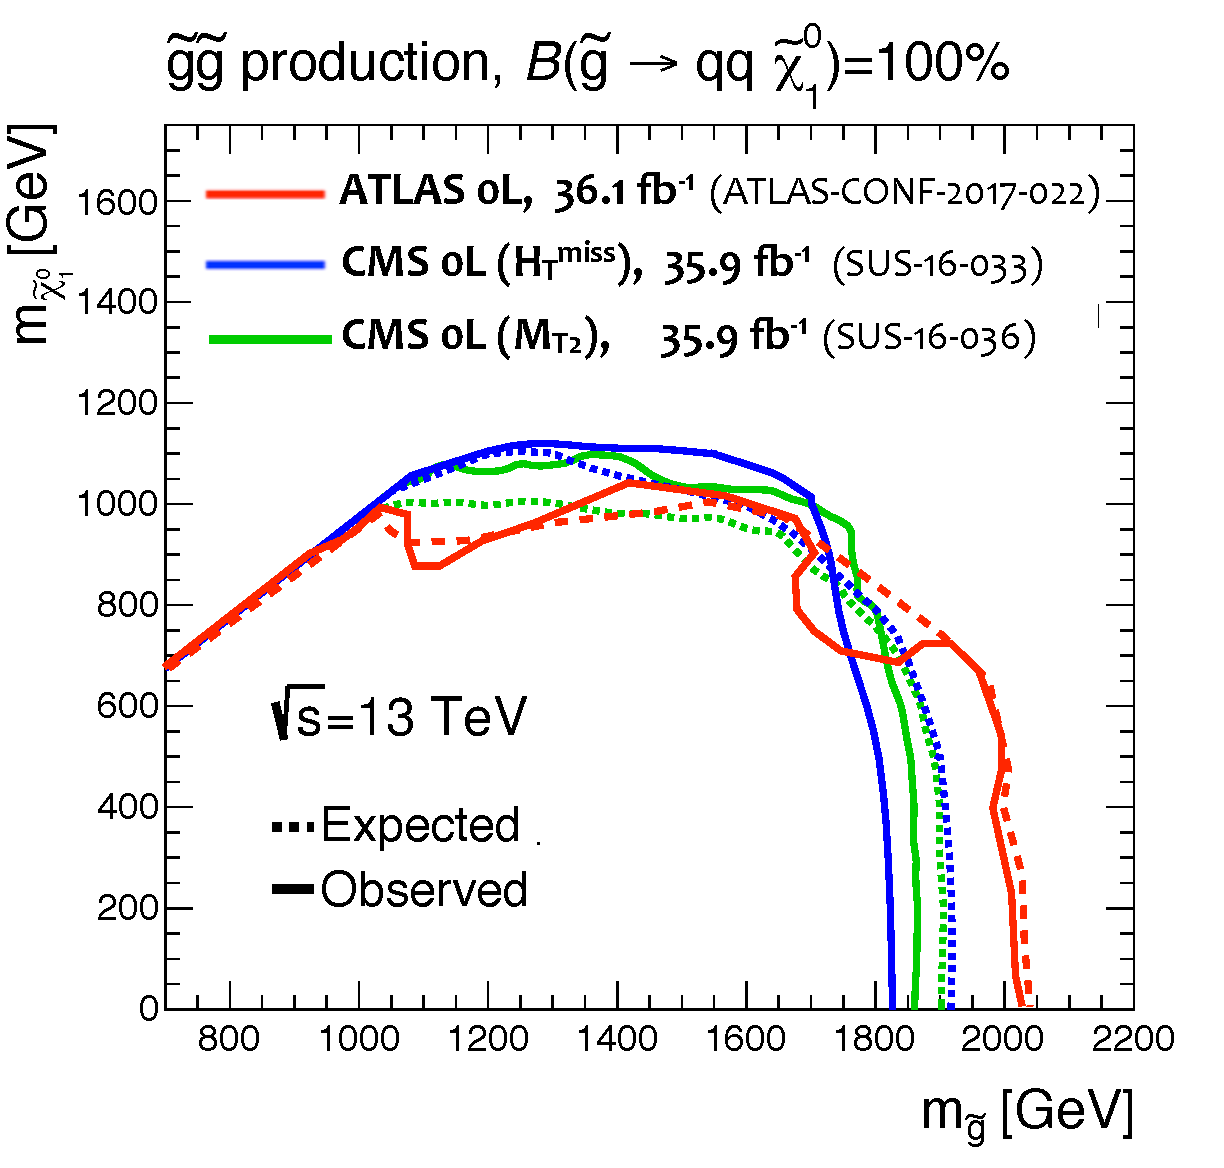
\includegraphics[width=0.48\textwidth]{figures/Introduction/LHC_SUSY_GG_direct_36.pdf}}
    \subfigure[]{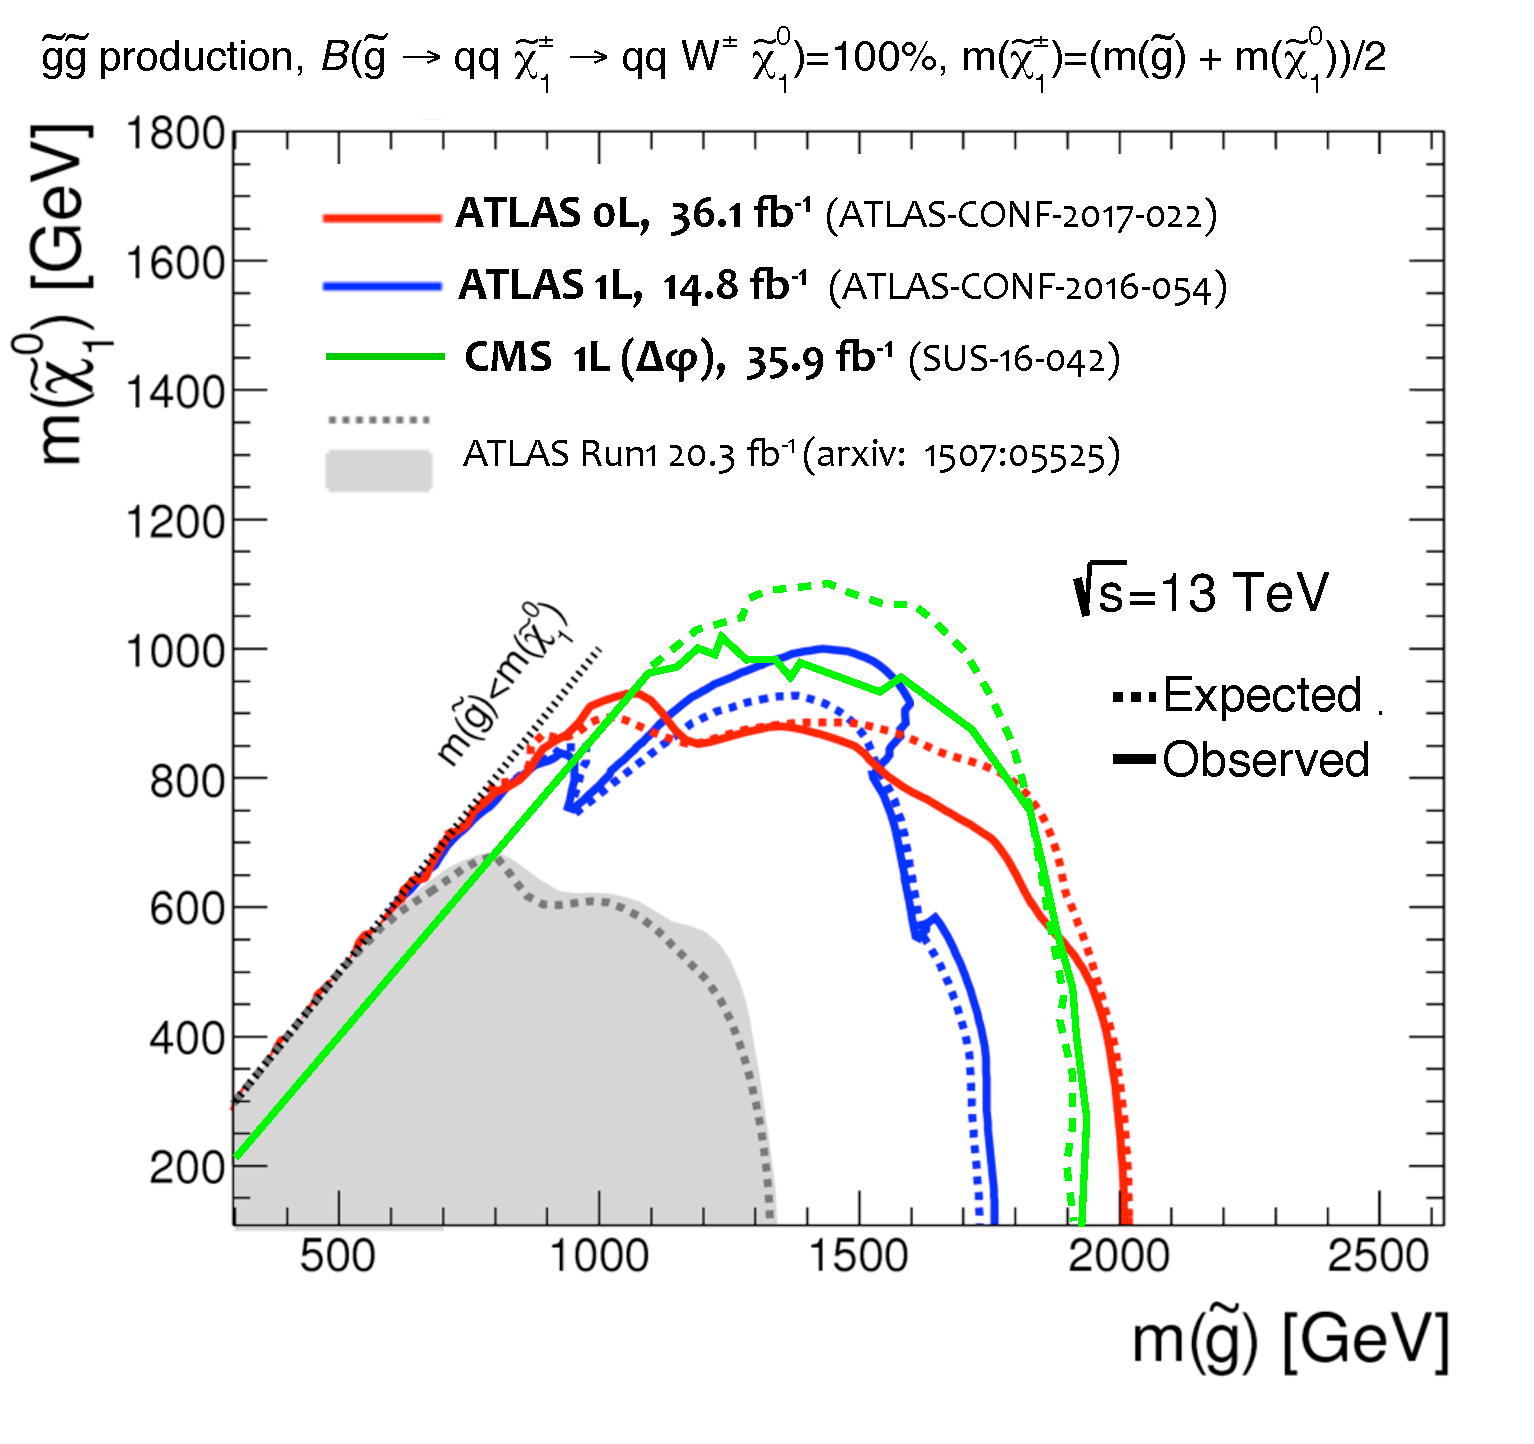
\includegraphics[width=0.48\textwidth]{figures/Introduction/LHC_SUSY_GG_1step_36.pdf}}
    \caption{Up-to-date constraints set by ATLAS and CMS on (a) direct gluino decay: $\tg \ra q \bar{q} \tLSP$, and (b) 1-step chargino-mediated gluino decay: $\tg \ra q\bar{q} \tchic$ with the mass being in the middel between gluino and the LSP.}
    \label{fig::Introduction::LHCLimitGG}
\end{figure}


Gluino decaying with top quarks addresses particular importance since it can be enhanced by the light stop which is motivated by naturalness. They are exclusively searched with dedicated signal regions, and the resultant limit in given in Fig. \ref{fig::Introduction::LHCLimitGtt}.

\begin{figure}[h]
  \centering
    \subfigure[]{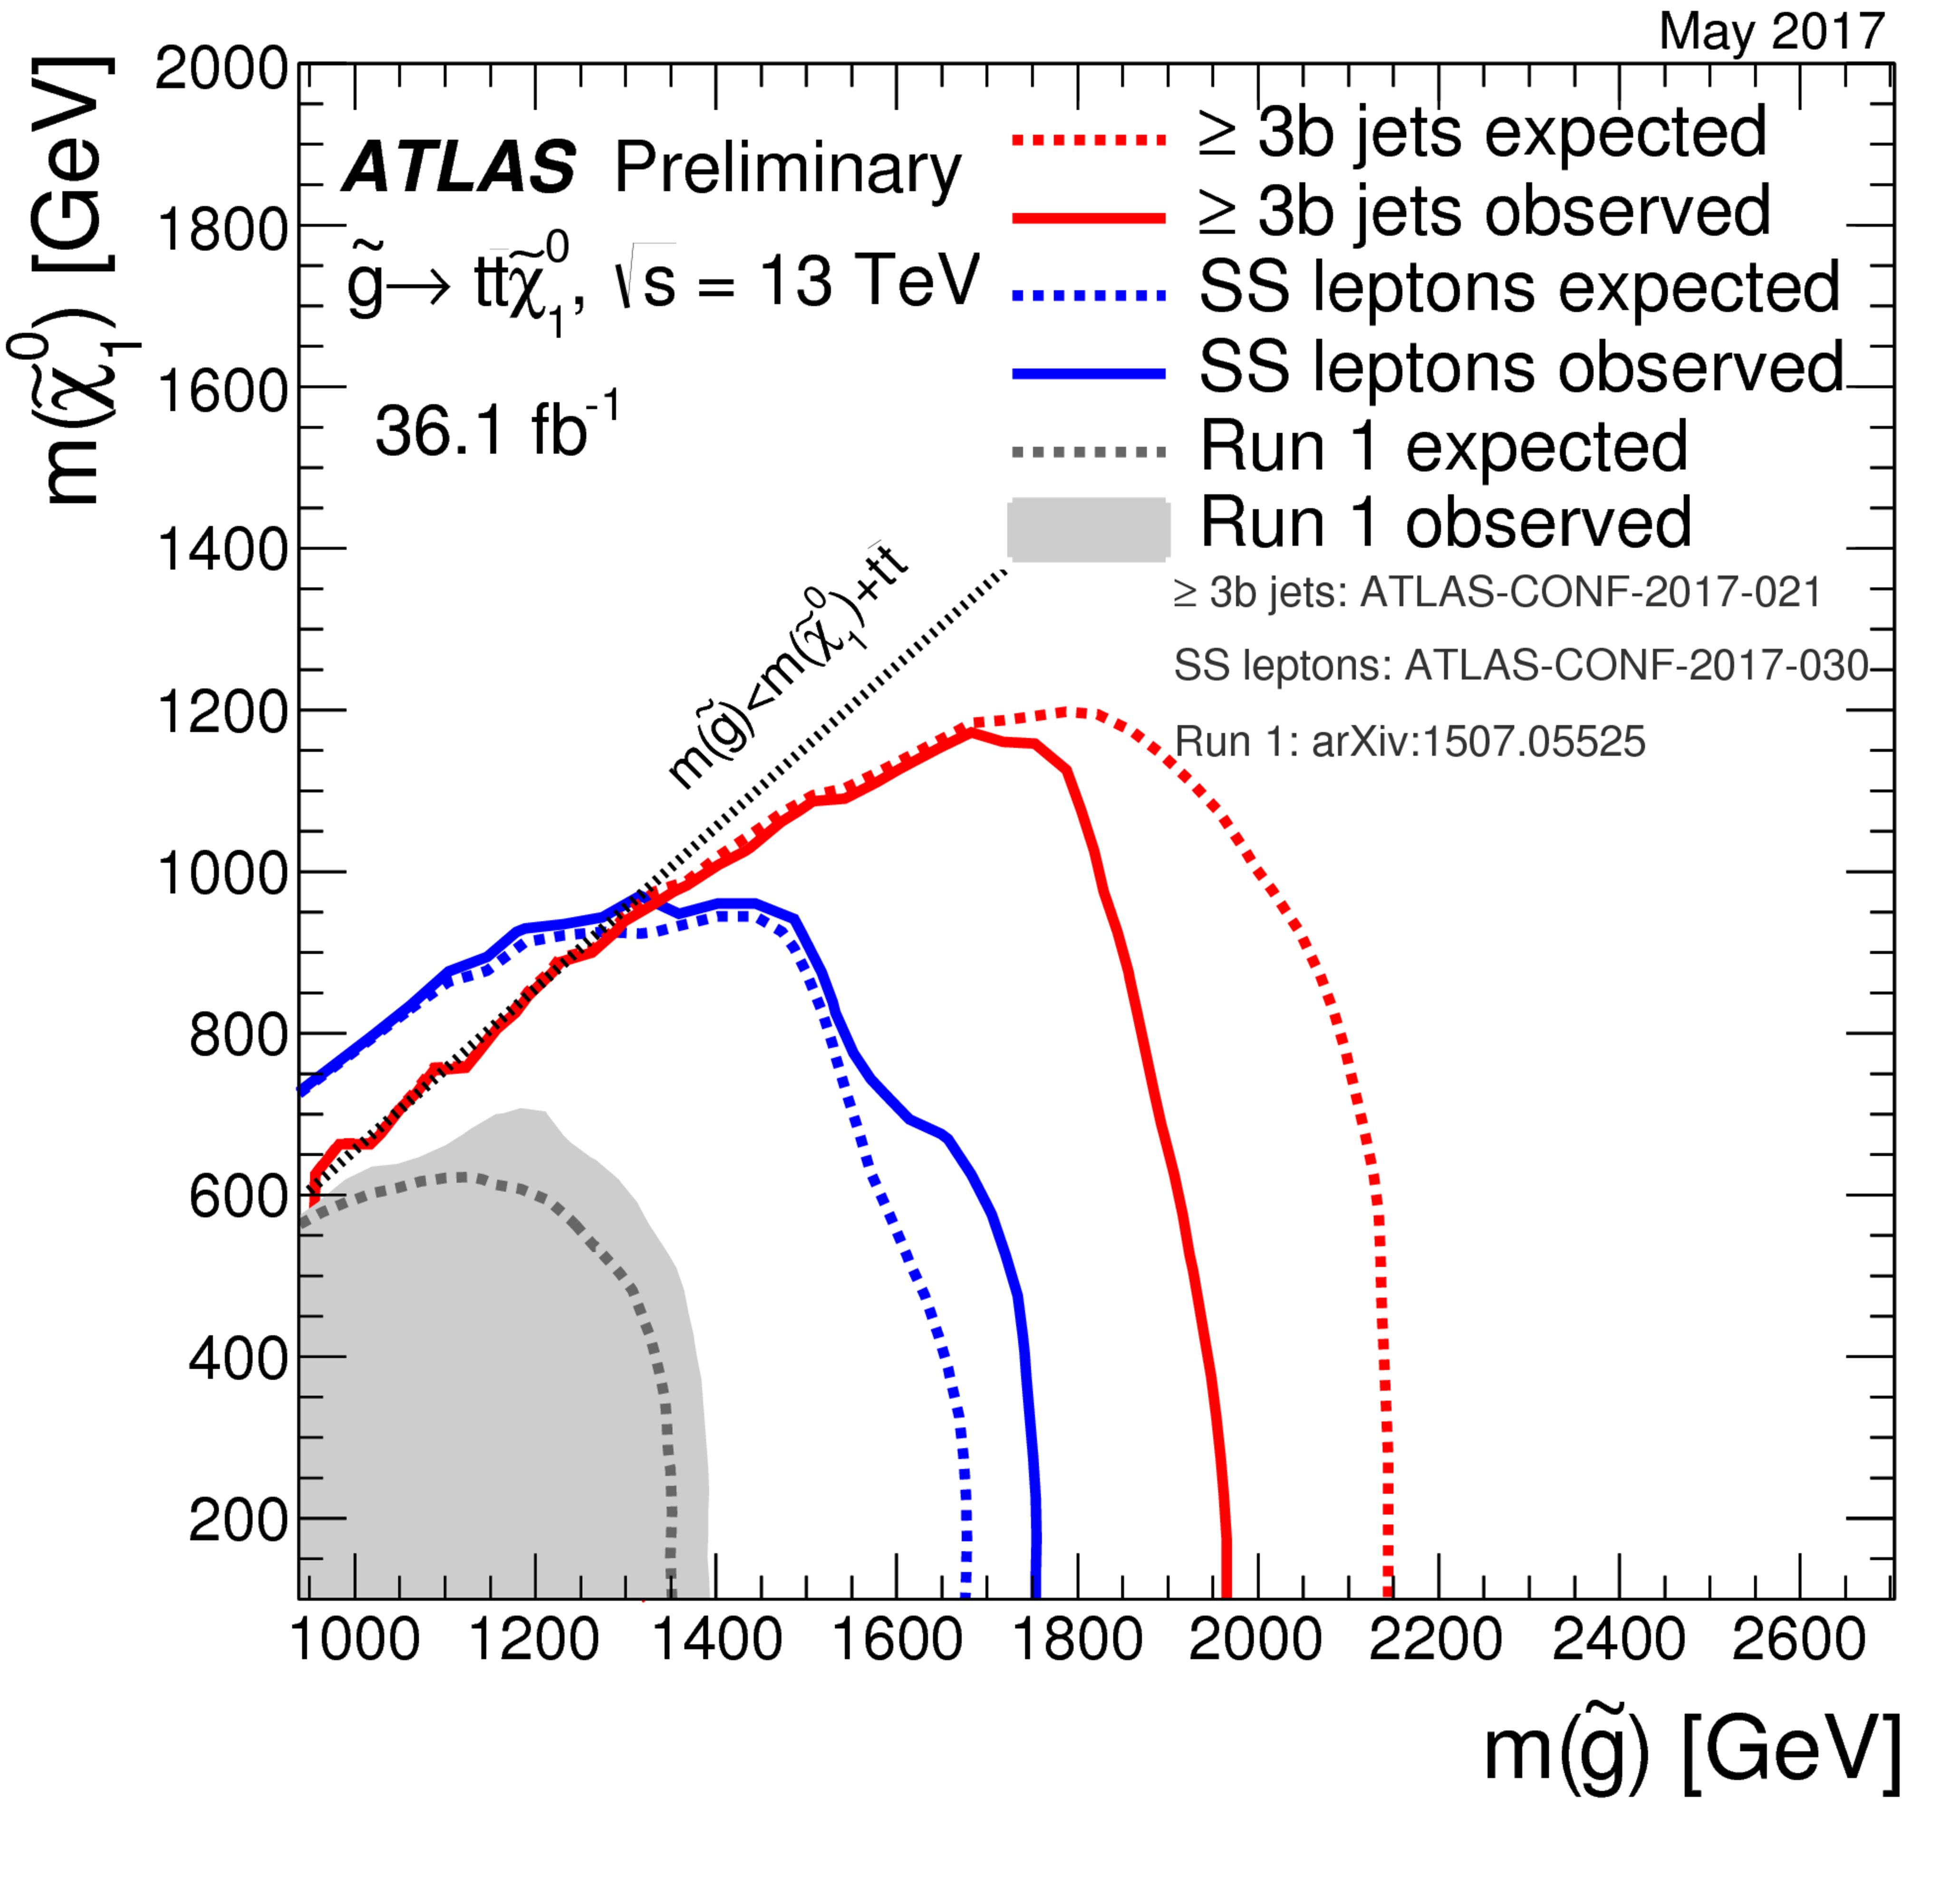
\includegraphics[width=0.48\textwidth]{figures/Introduction/ATLAS_SUSY_Gtt_36.pdf}}
    \subfigure[]{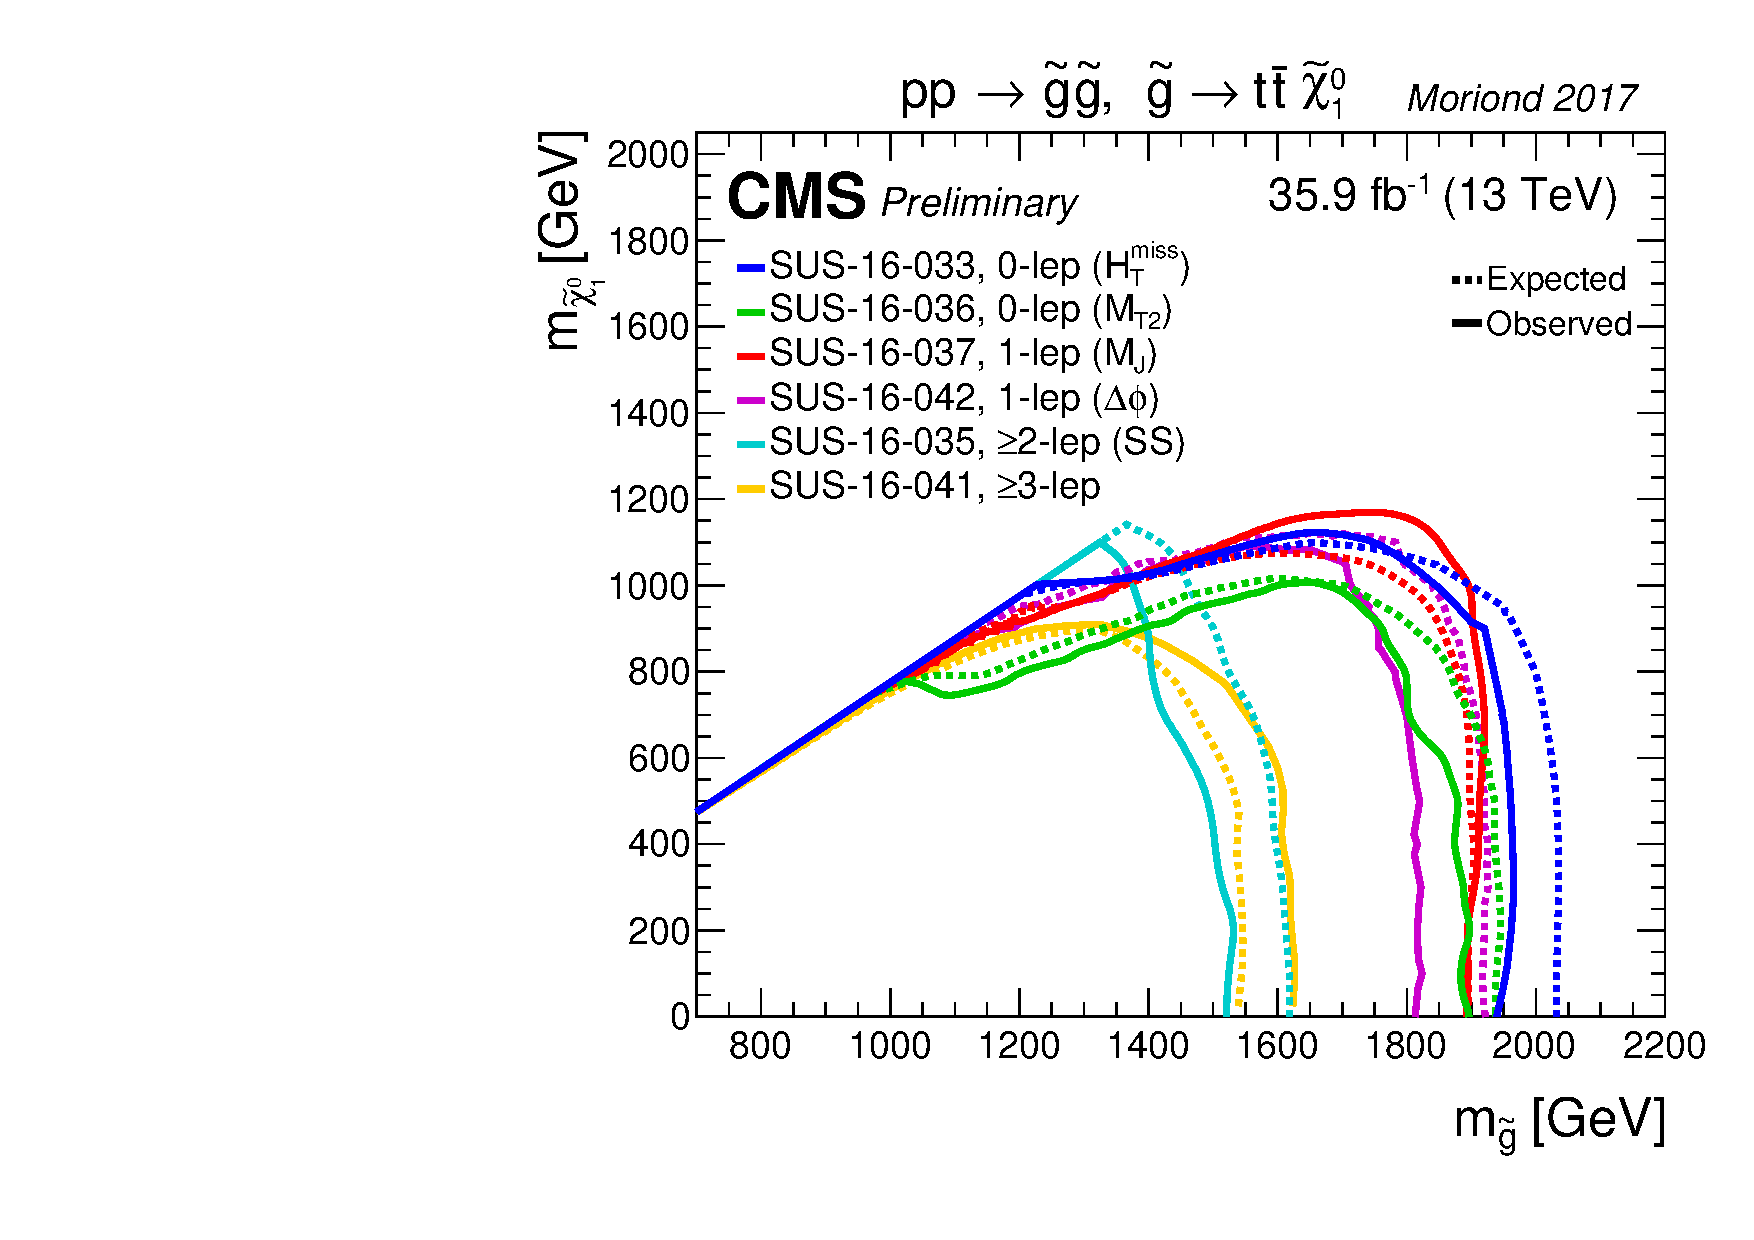
\includegraphics[width=0.48\textwidth]{figures/Introduction/CMS_gg_tt_36.pdf}}
    \caption{Up-to-date constraints set by (a) ATLAS and (b) CMS on direct gluino decay with associated top quarks: $\tg \ra t\bar{t} \tLSP$.}
    \label{fig::Introduction::LHCLimitGtt}
\end{figure}


\paragraph{Squarks}
Sine stop claims particular motivation for naturalness among all squarks, 
the analyzes are dedicatedly designed to address to wide range of decays of mass configurations.
The strongest limits are provided by LHC, and Fig. \ref{fig::Introduction::LHCLimitStop} presents the exlusion limits obtained by ATLAS and CMS on the most typical decay scenario $\ttop \ra t \tilde{\chi}_1^0$.
Upto about $400\gev \sim 1\tev$ of stop mass is excluded for depending on the mass splitting, which is similar to the other decay models as well including $\ttop \ra b \tchic$.

\begin{figure}[h]
  \centering
    \subfigure[]{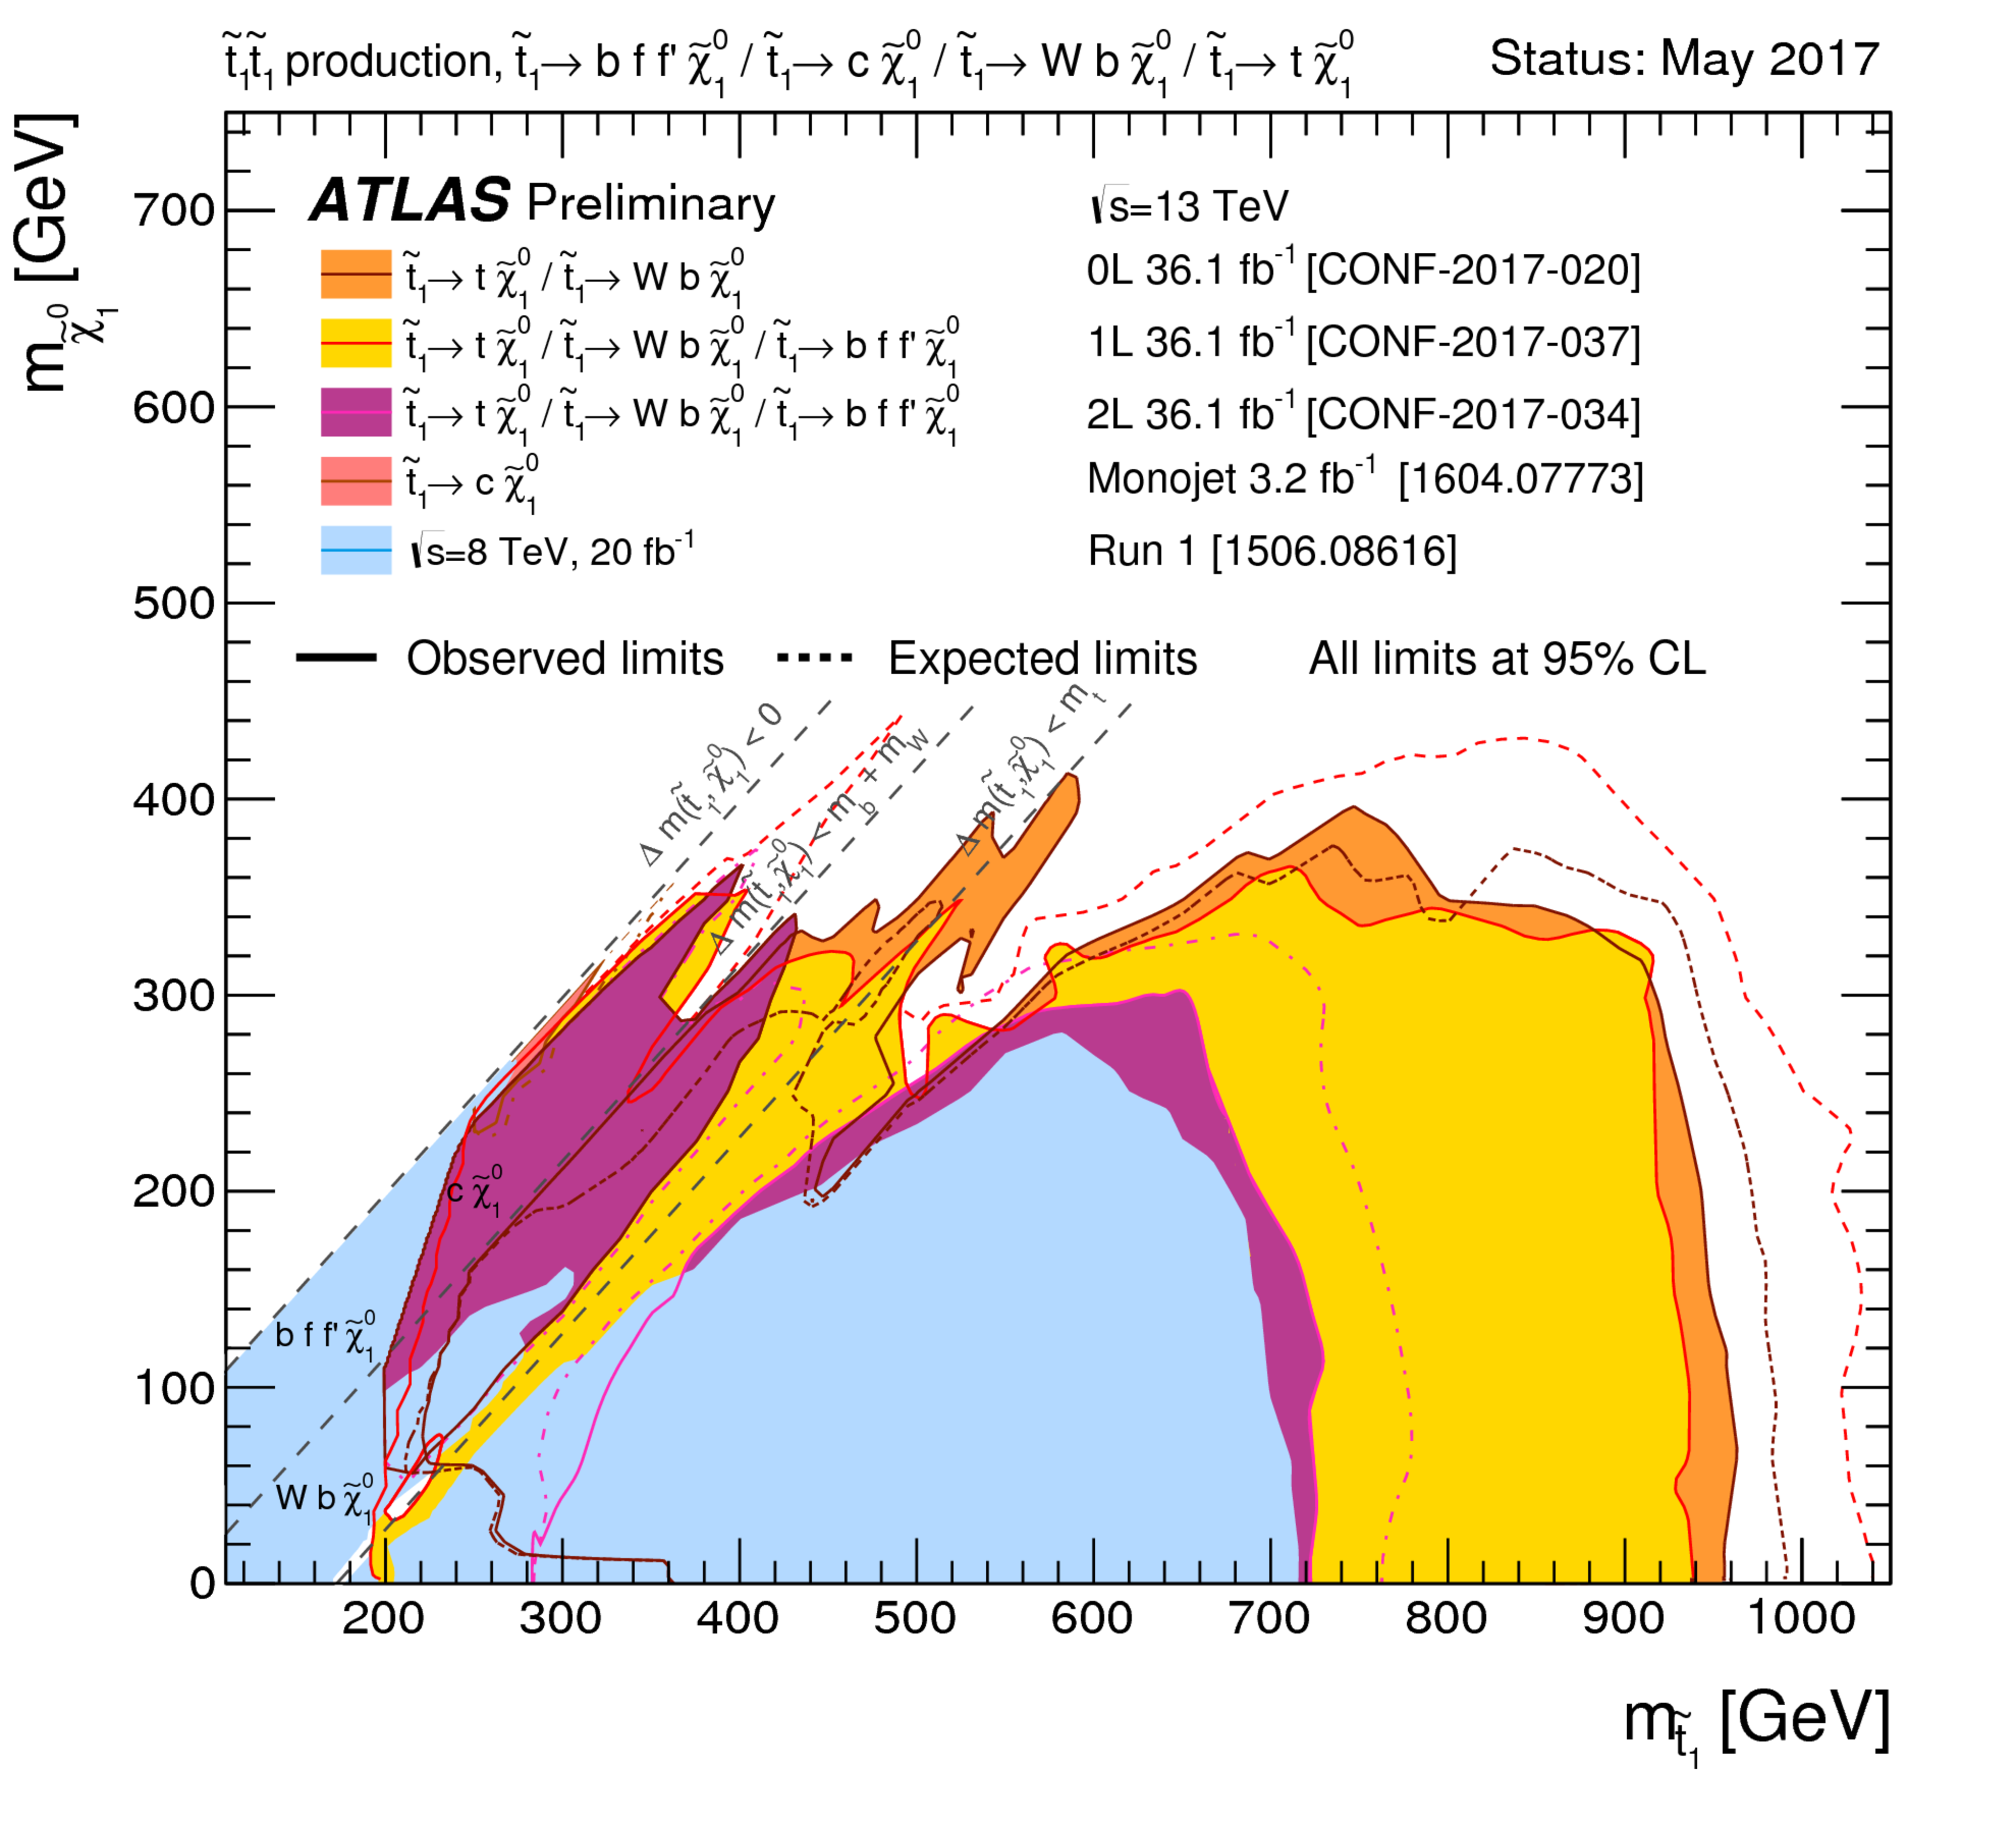
\includegraphics[width=0.48\textwidth]{figures/Introduction/ATLAS_SUSY_Stop_tLSP.pdf}}
    \subfigure[]{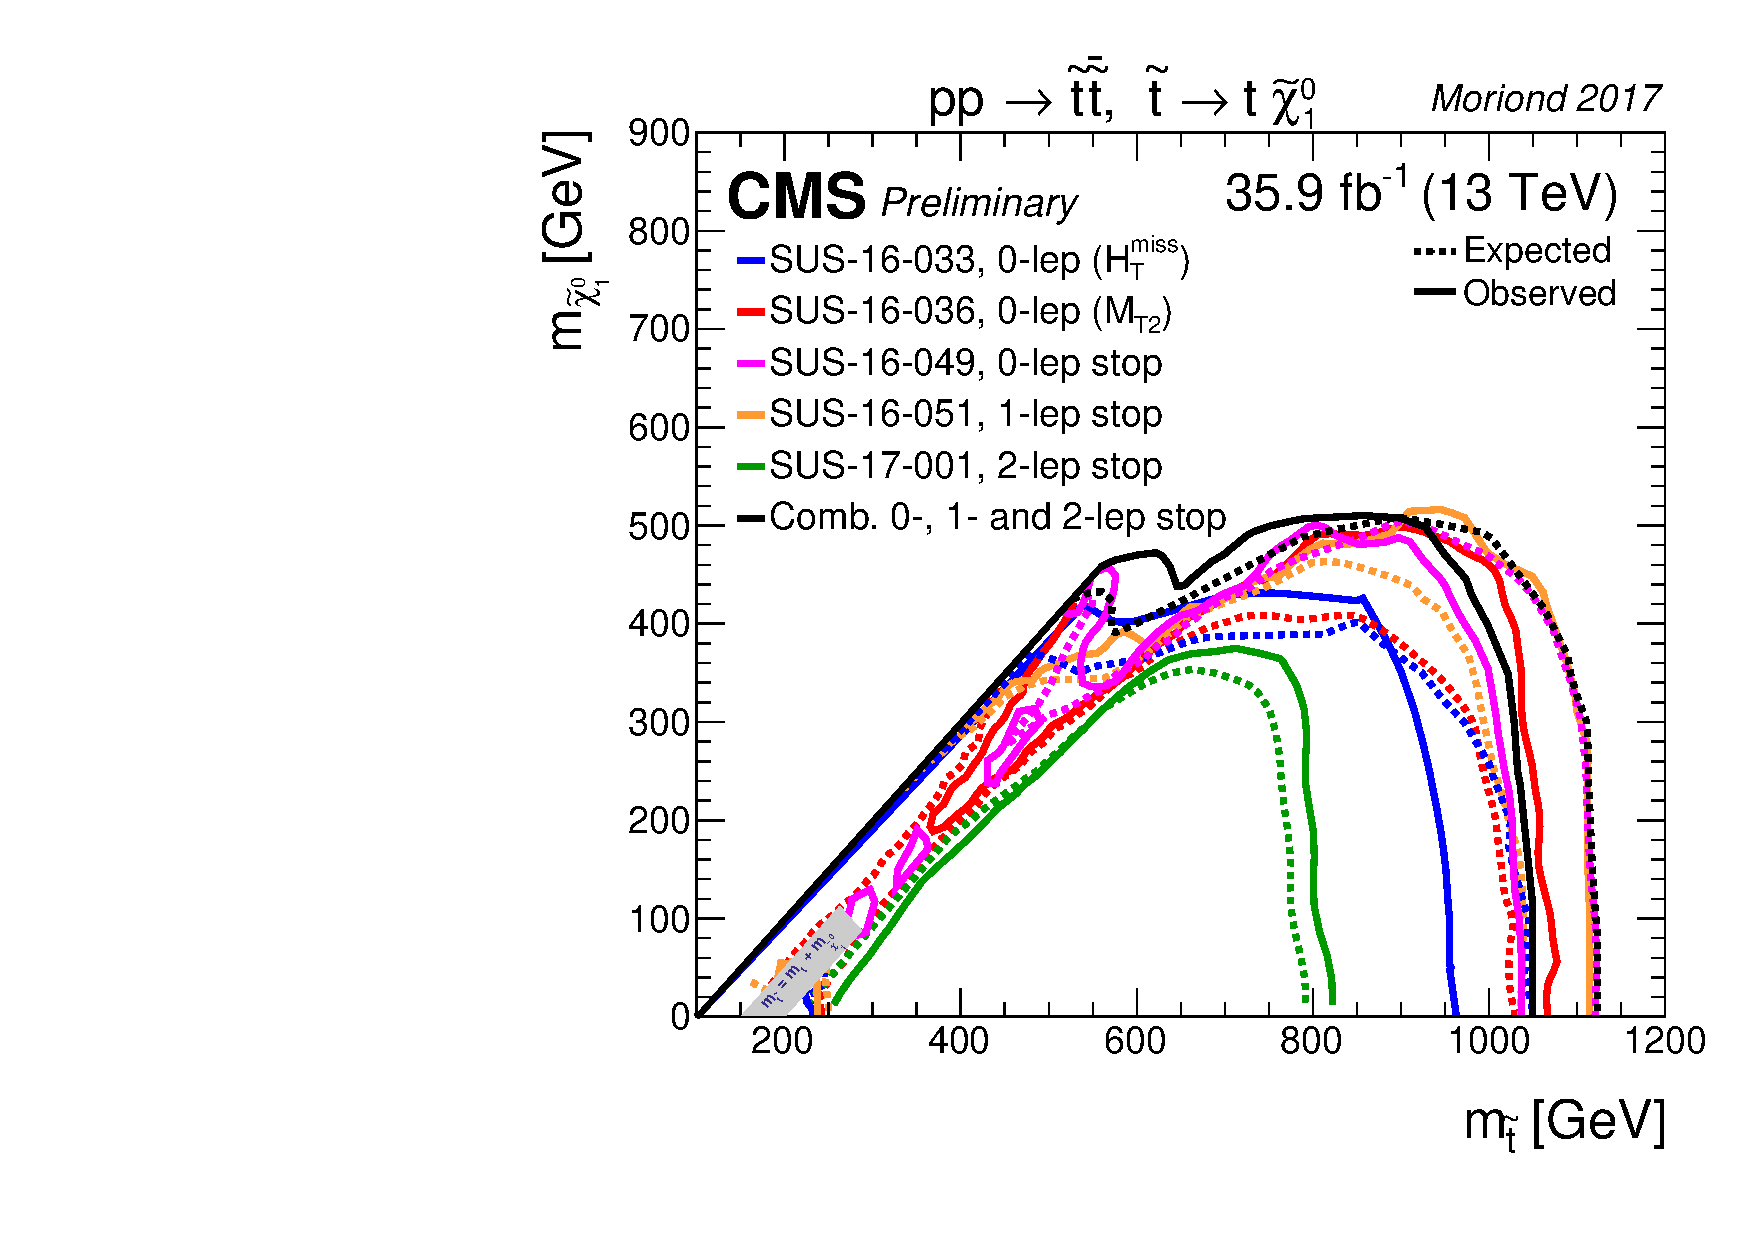
\includegraphics[width=0.48\textwidth]{figures/Introduction/CMS_stop_36.pdf}}
    \caption{Up-to-date constraints set by (a) ATLAS and (b) CMS on stop pair production with direct decay $\ttop \ra t \tilde{\chi}_1^0$.}
    \label{fig::Introduction::LHCLimitStop}
\end{figure}



\paragraph{Electroweak Gauginos}
A number of searches have been performed in LEP, Tevatron and LHC, and the LHC result set the majority of the current storngest limits. The target signatures are mainly pair produced NLSPs ($\tchic$ or $\tchin$) directly decaying to LSP, where wino dominated NLSP, bino-dominated LSP, and decoupled squarks are commonly assumed.
\footnote{Under the decoupled squark scenario, bino production is strongly suppressed.}
The signal regions typically require multiple leptons and large missing ET in the final states.
The exclusion limits set by ATLAS and CMS is shonw in Fig. \ref{fig::Introduction::LHCLimitEWKino}.
About upto $500\gev$ of NLSP mass is excluded for cases with large NLSP-LSP mass splitting, and $200-250\gev$ for small mass splitting.  \\


\begin{figure}[h]
  \centering
    \subfigure[]{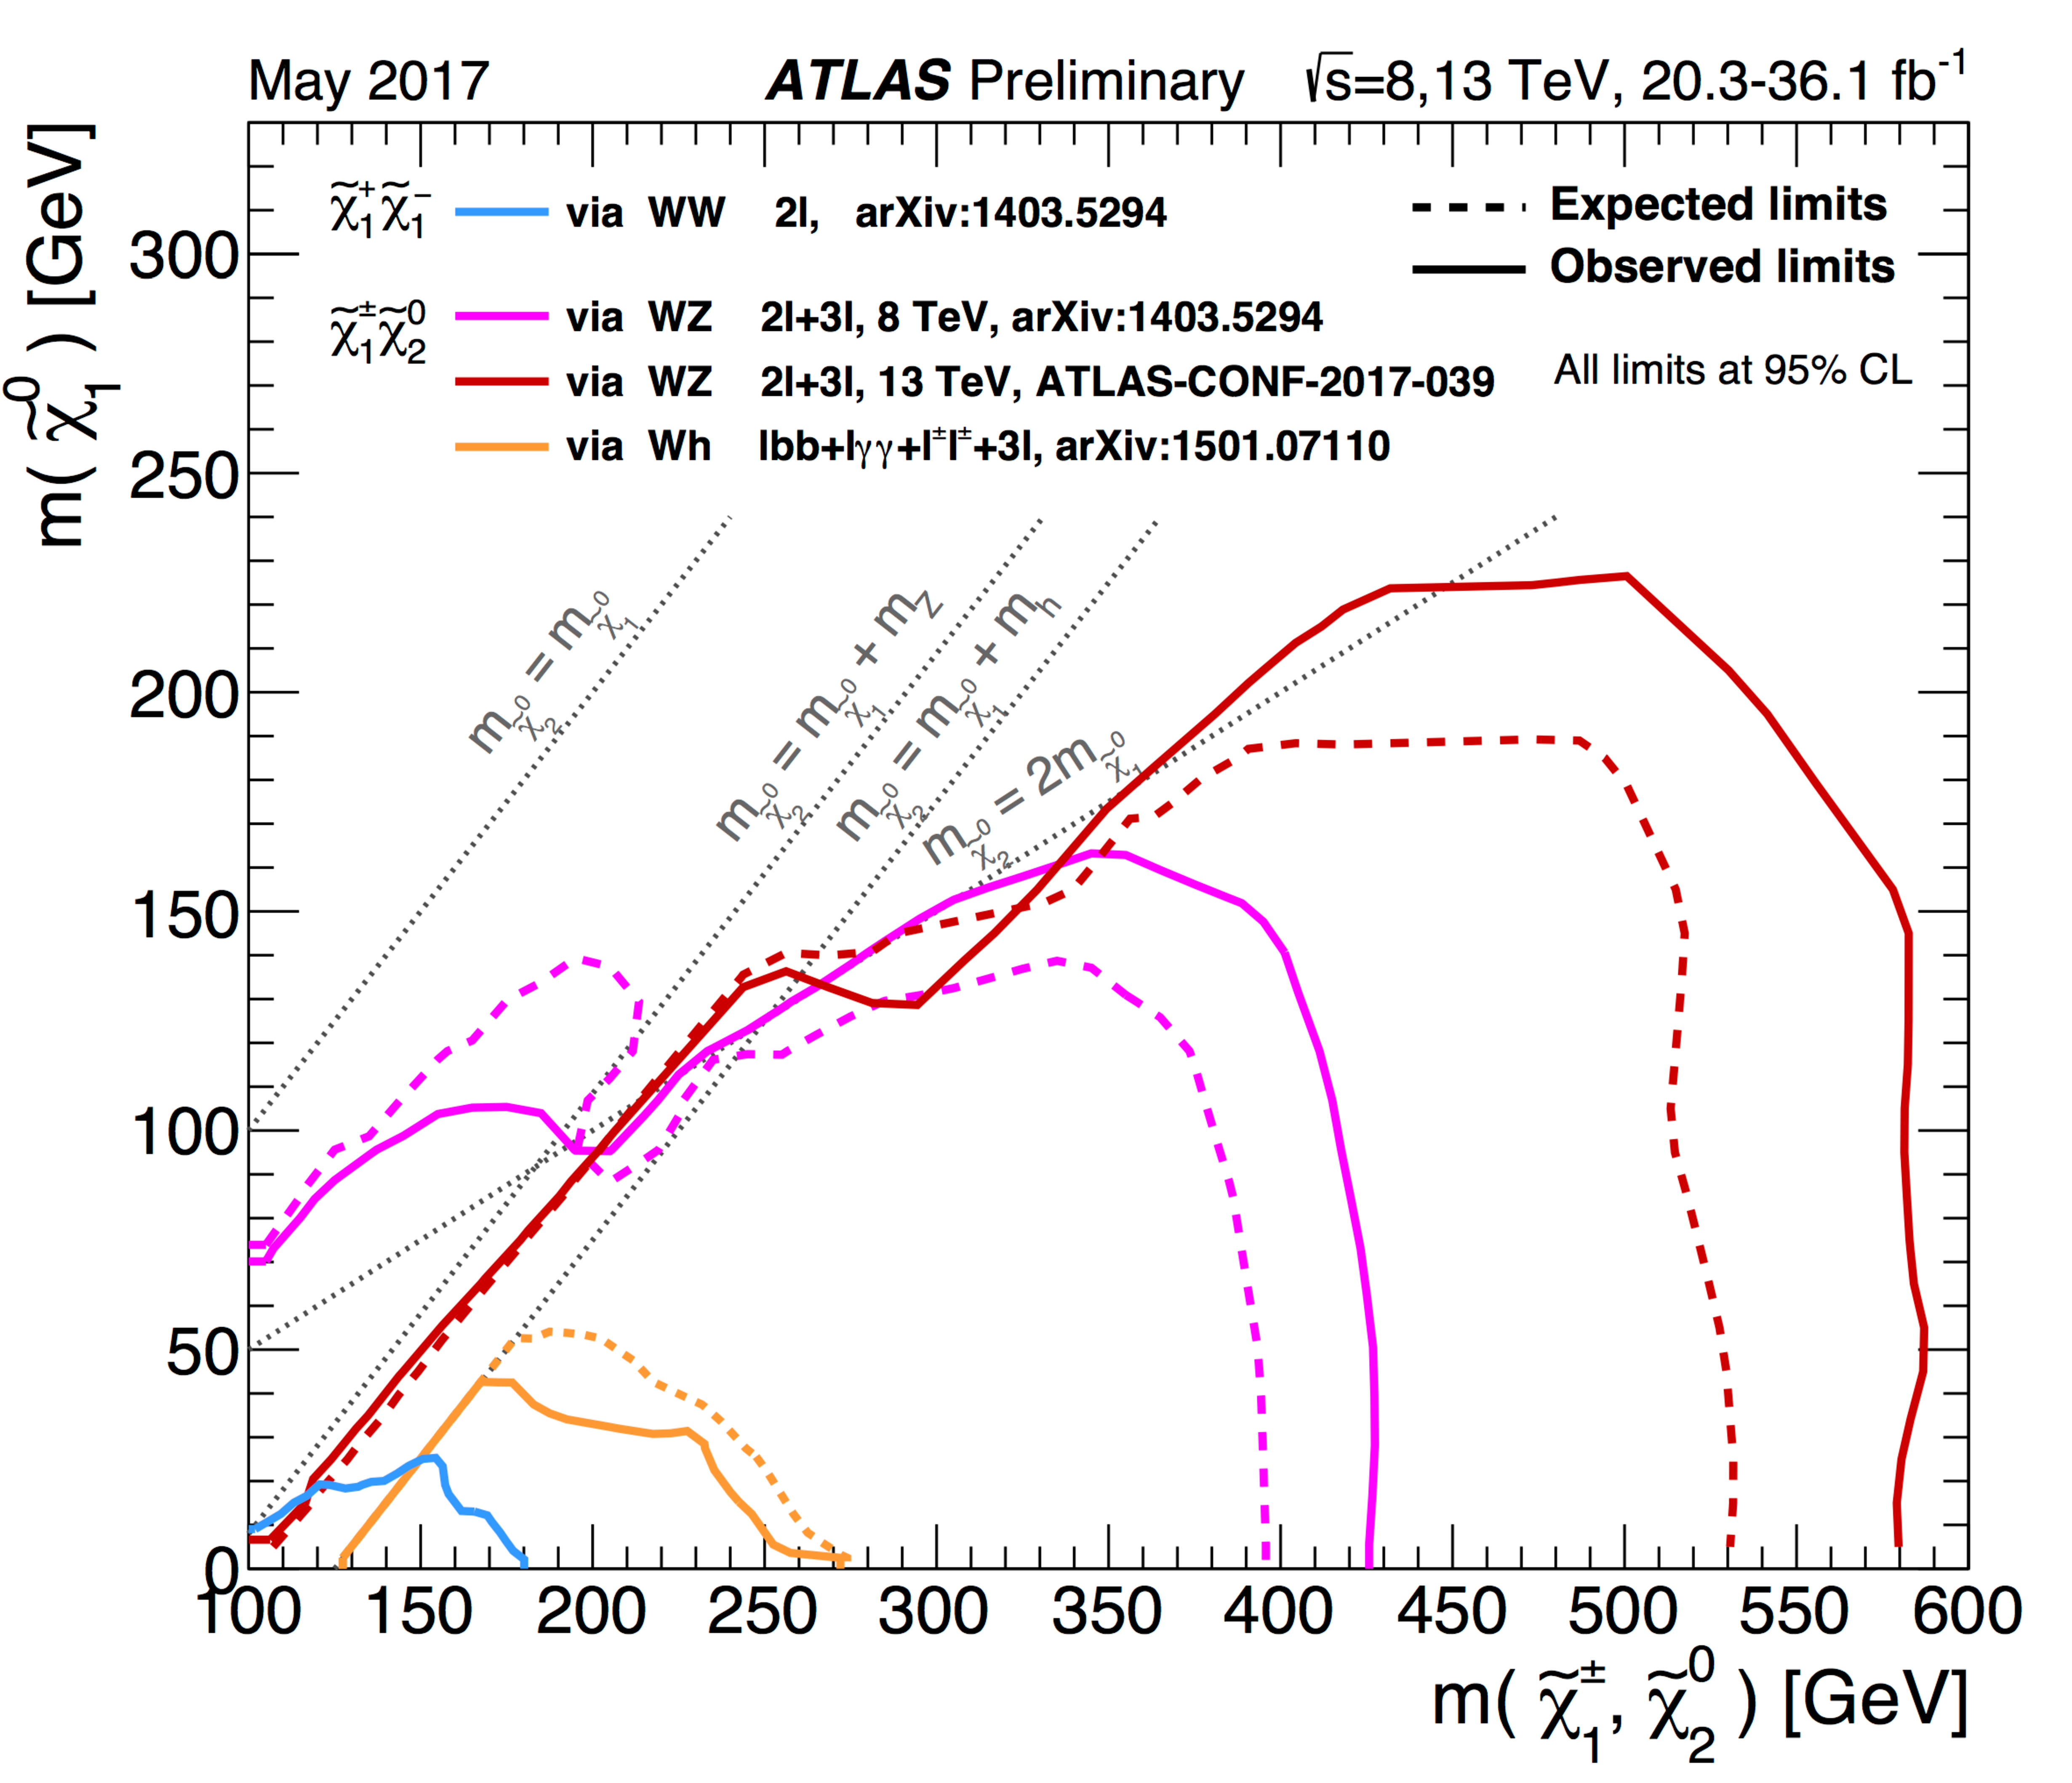
\includegraphics[width=0.48\textwidth]{figures/Introduction/ATLAS_EWgaugino_WZh_36.pdf}}
    \subfigure[]{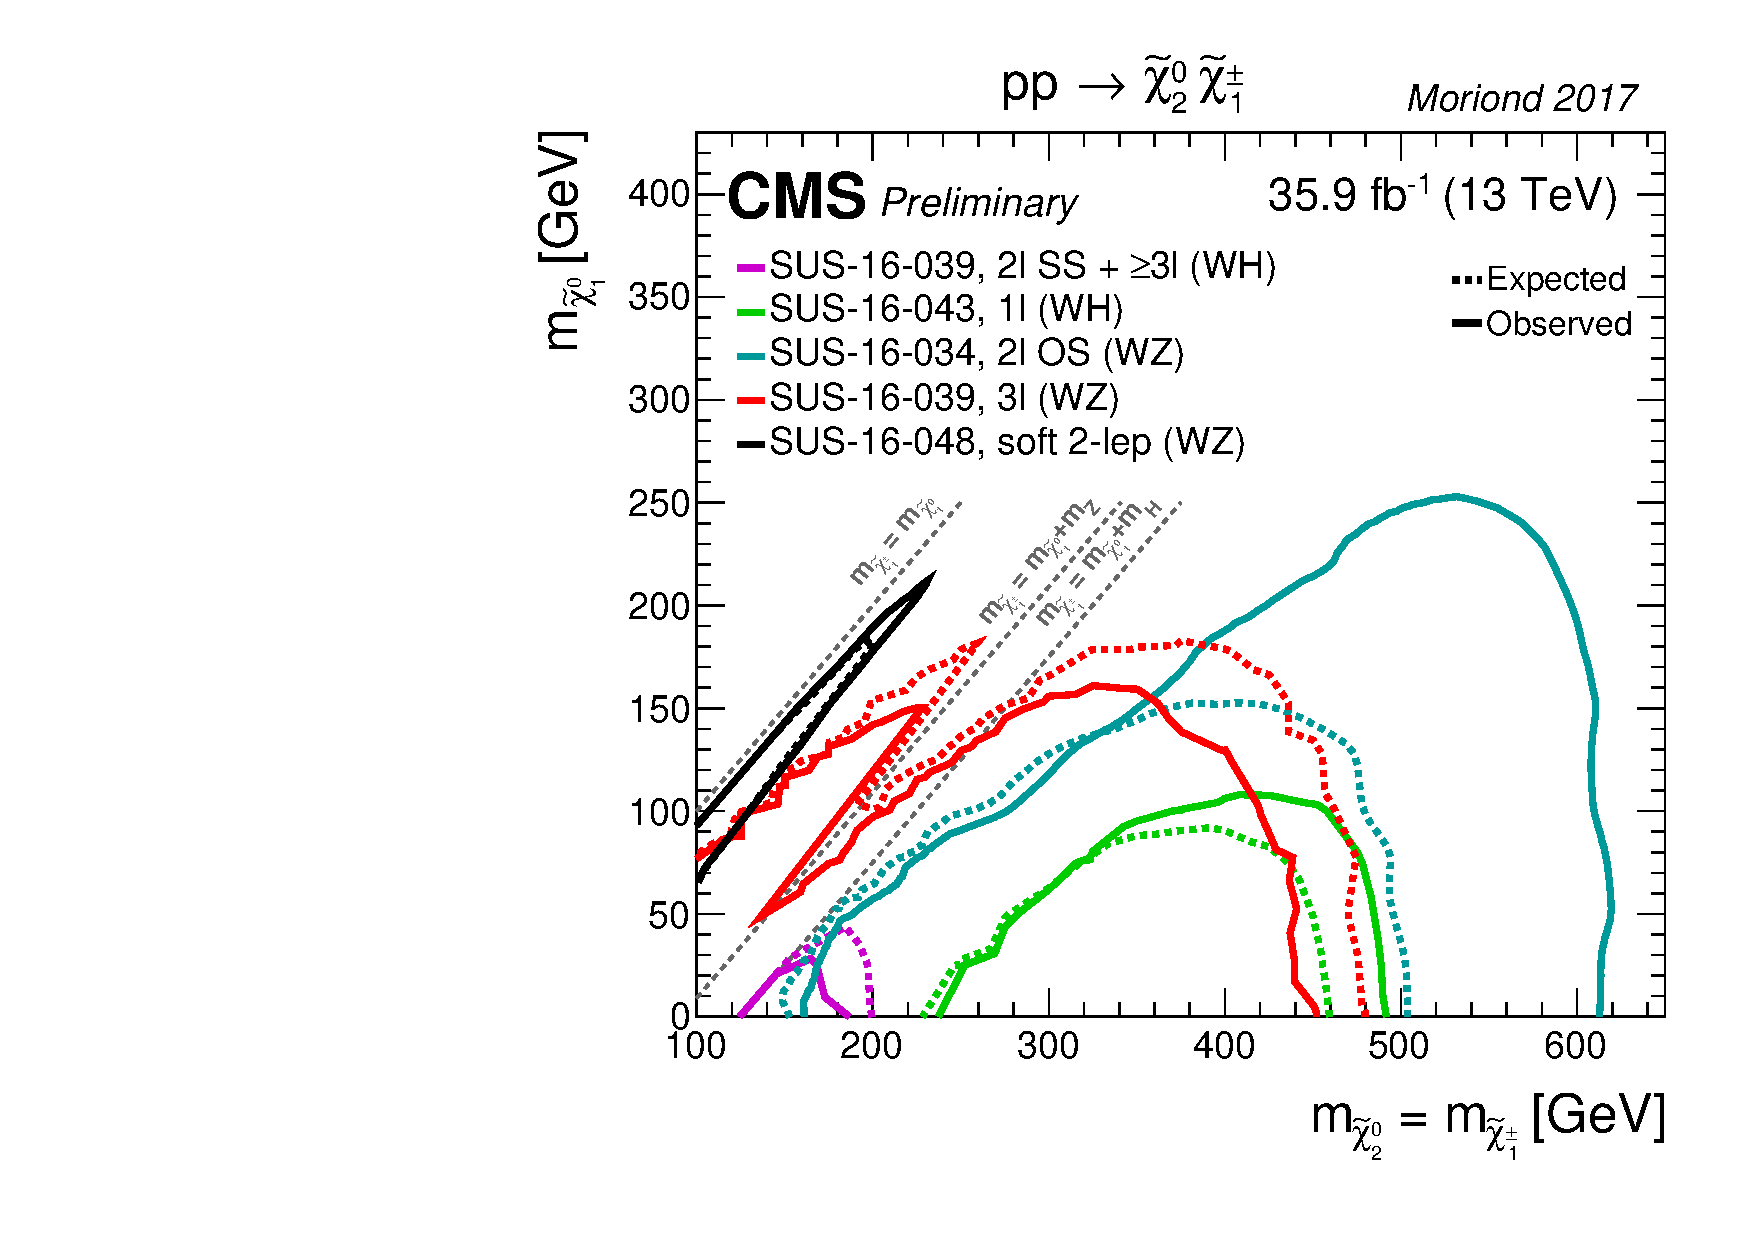
\includegraphics[width=0.48\textwidth]{figures/Introduction/CMS_EWgaugino_WZh_36.pdf}}
    \caption{Up-to-date constraints set by (a) ATLAS and (b) CMS on direct EW gaugino production with decays via $W/Z/h$.}
    \label{fig::Introduction::LHCLimitEWKino}
\end{figure}


The scenario with wino LSP is explored using a strikingly different approach. Since the mass splitting between NLSP wino-chargino and the wino-LSP is extremely compressed ($150 \sim 160\mev$), wino-chargino retains $O(\mathrm{ns})$ of moderately long lifetime, resulting the characterstic disappearing track signature where a visible charged track disappearing halfway in the tracker due to the decay. The result from ATLAS and CMS (Run1) is given in Fig. \ref{fig::Introduction::LHCLimitWino}.
The exlusion runs upto $300-500\gev$ of wino mass for the lifetime (or the NLSP-LSP mass splitting) predicted by MSSM. \\

\begin{figure}[h]
  \centering
    \subfigure[]{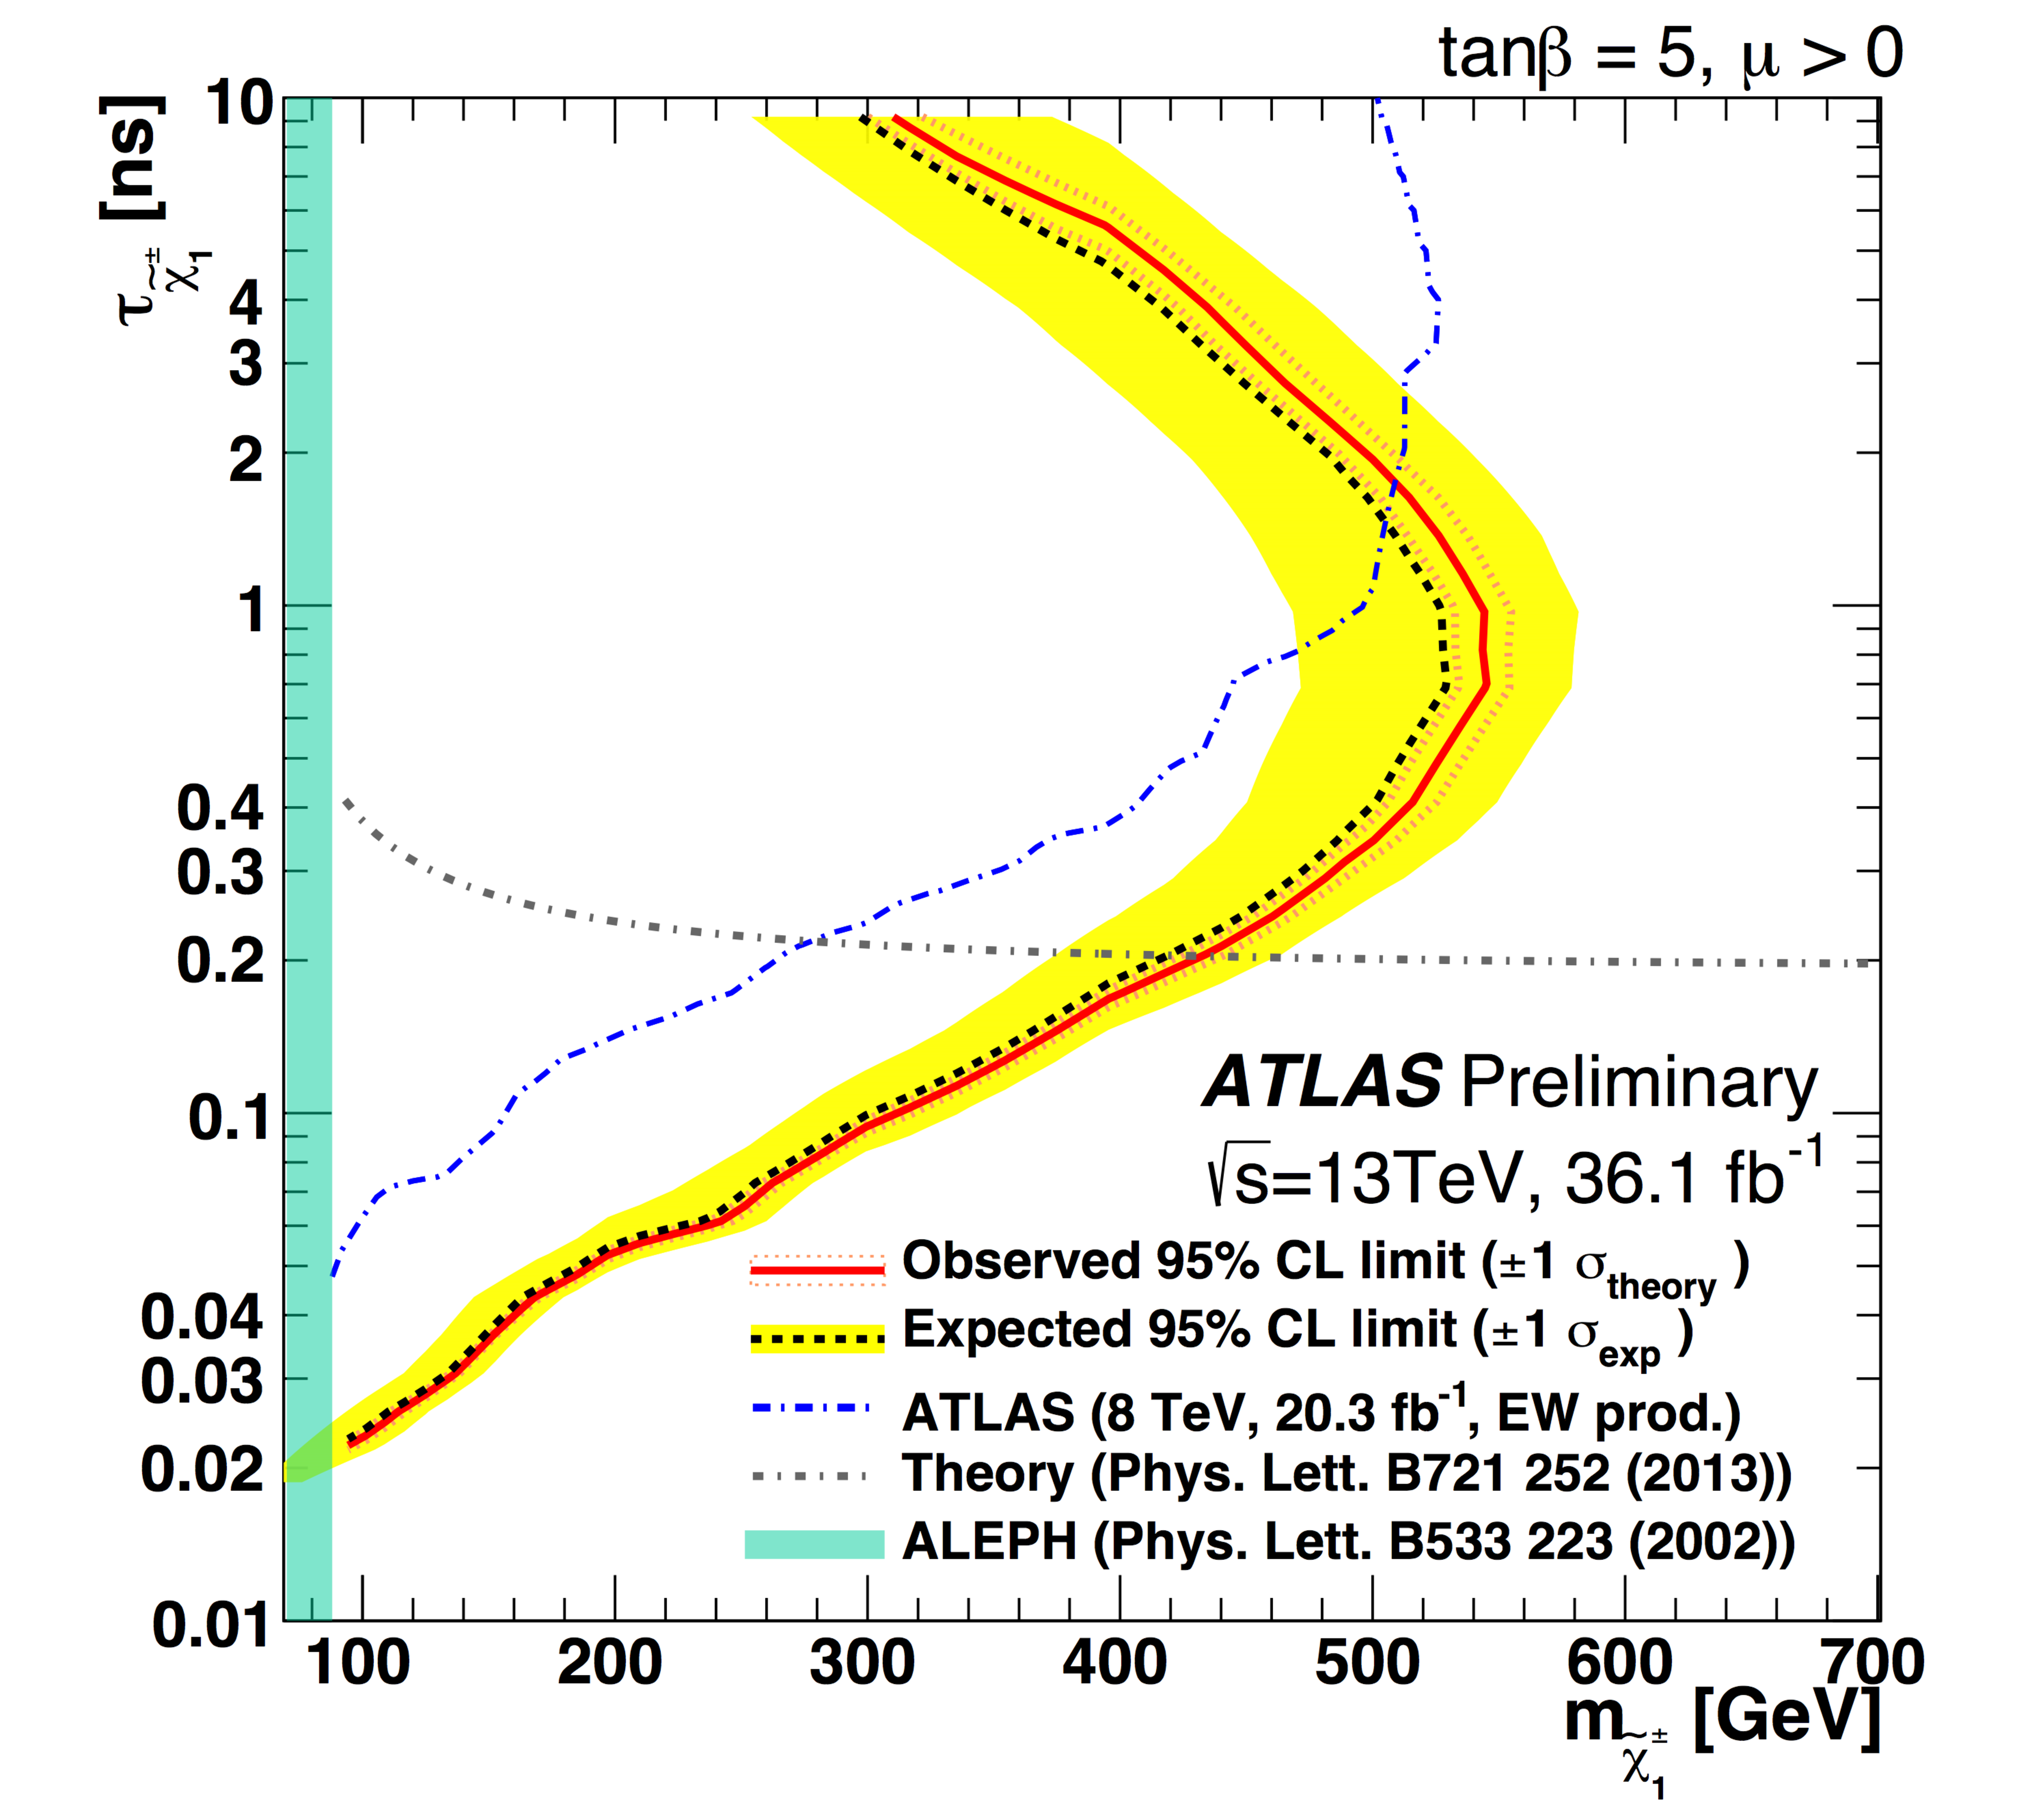
\includegraphics[width=0.48\textwidth]{figures/Introduction/ATLAS_SUSY_LLDT_36.pdf}}
    \subfigure[]{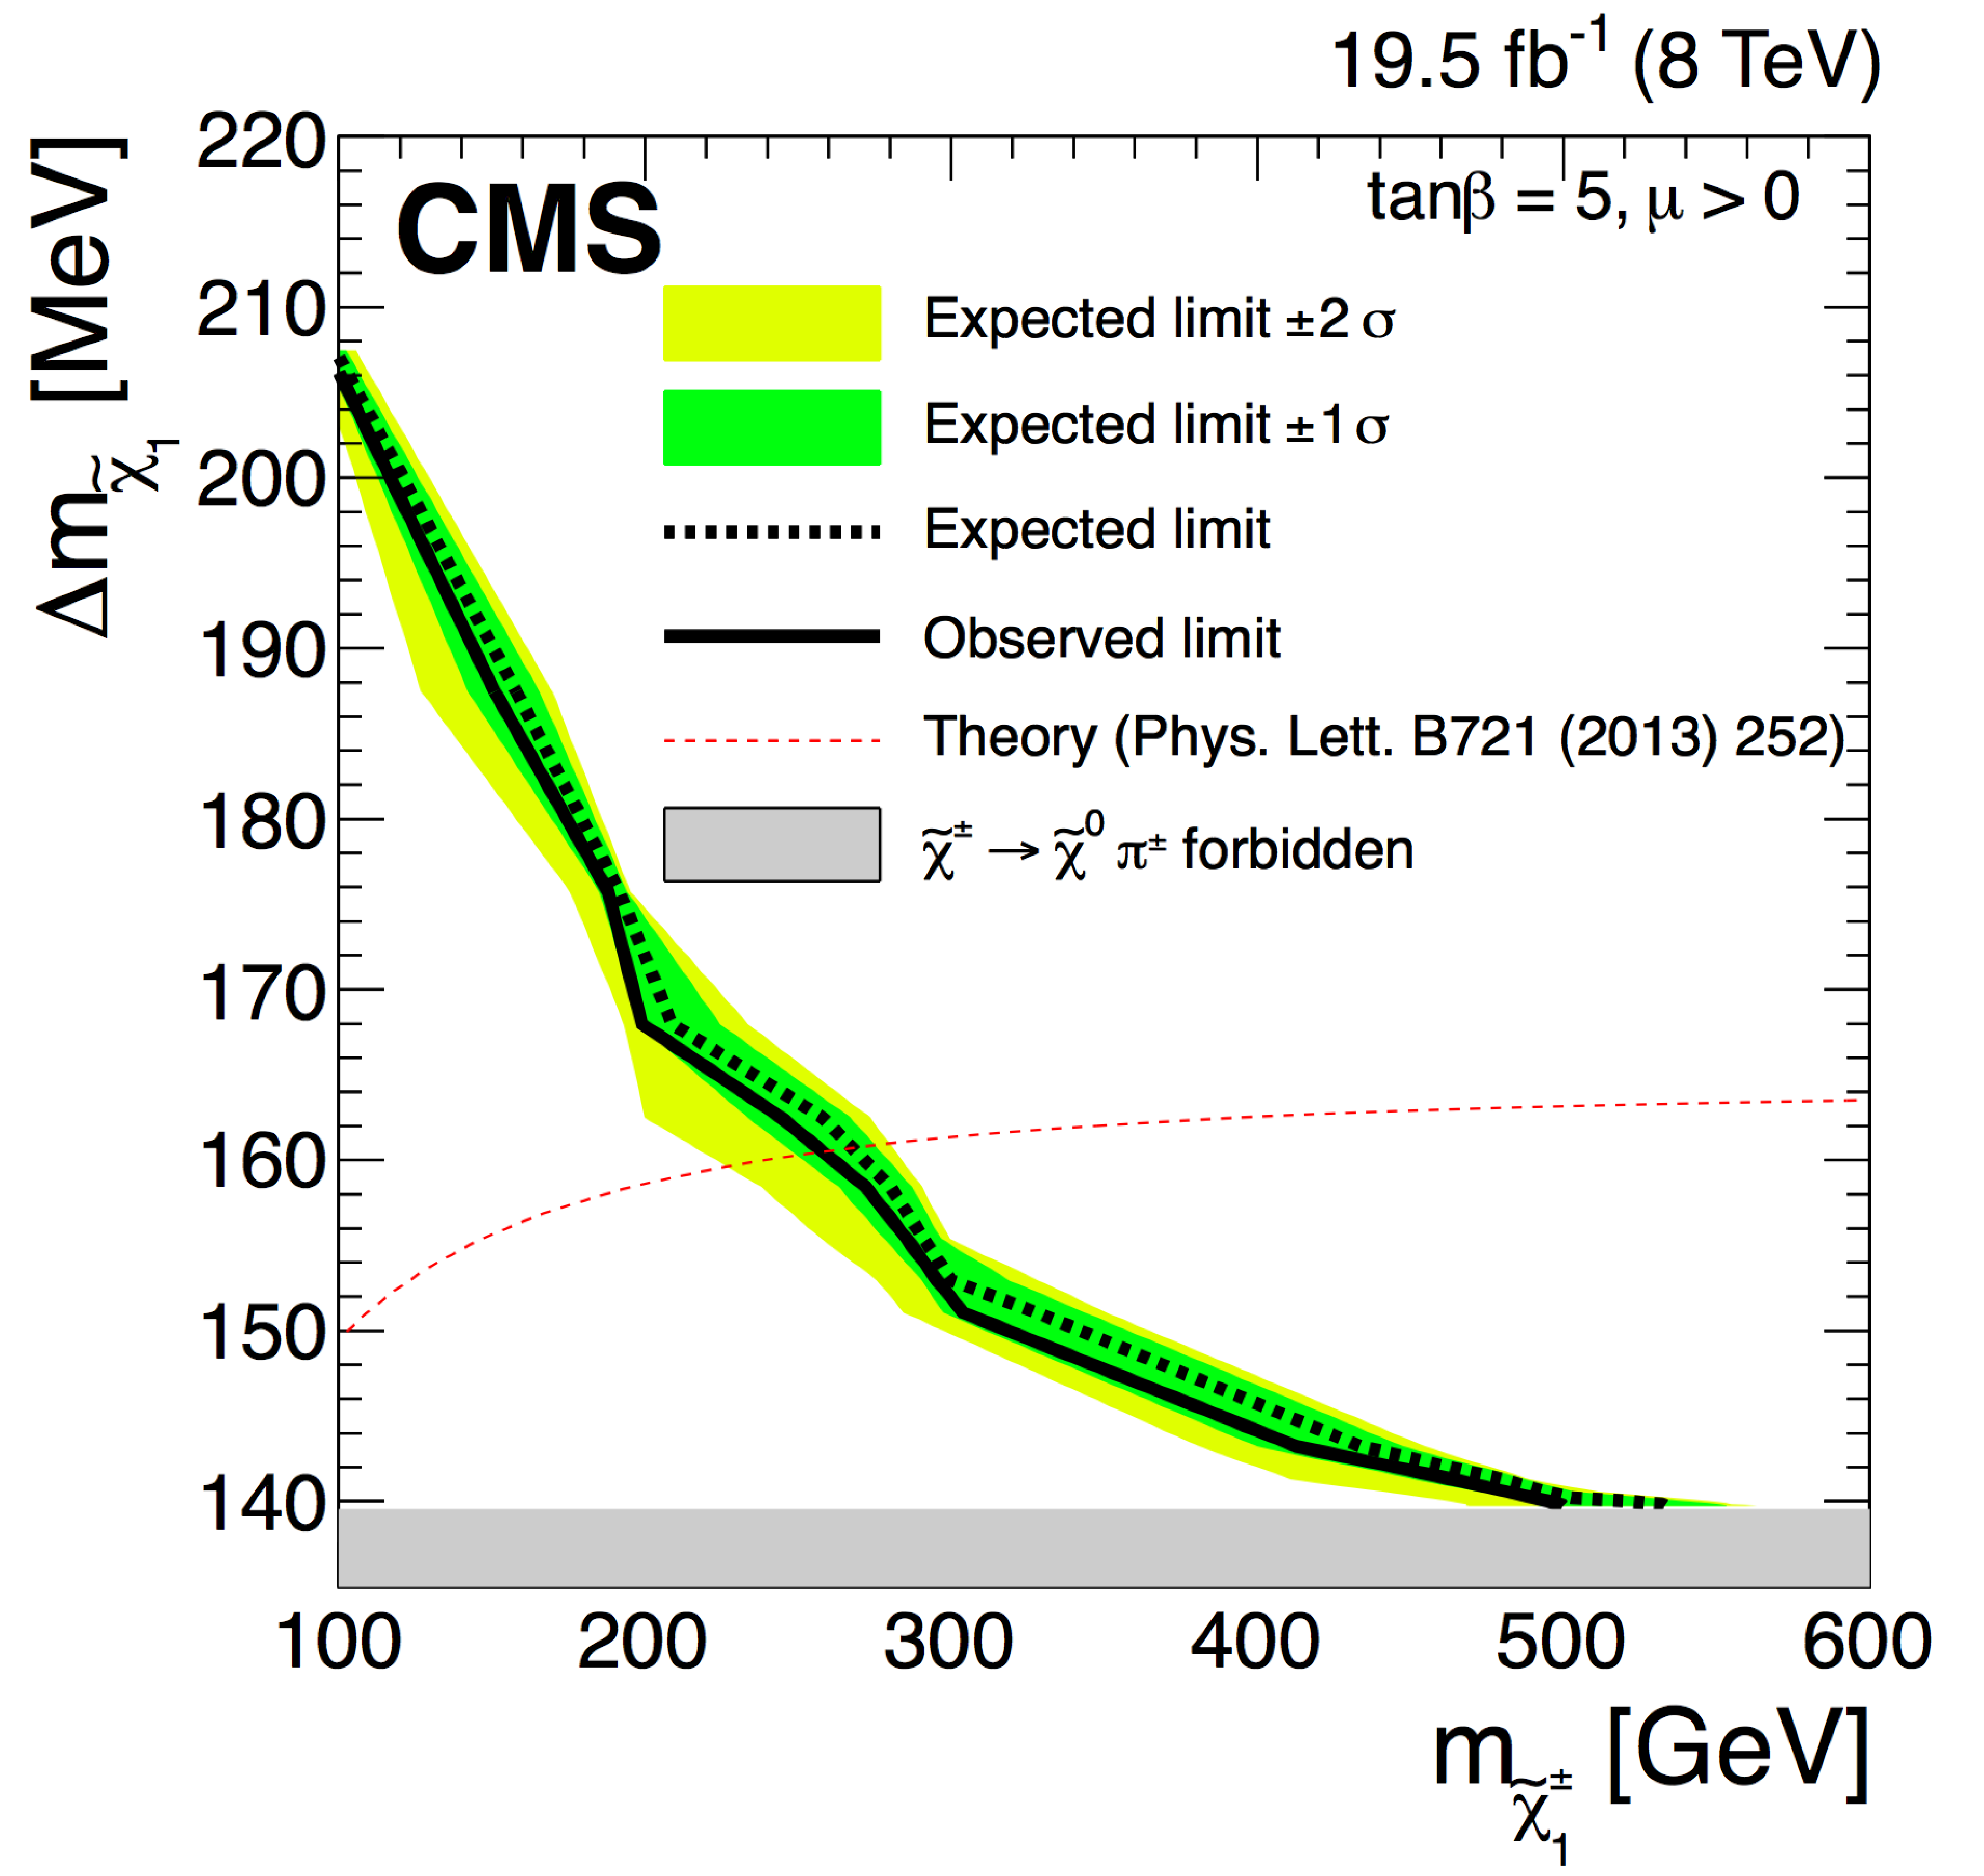
\includegraphics[width=0.48\textwidth]{figures/Introduction/CMS_SUSY_LLDT_Run1.pdf}}
    \caption{Constraints set on wino-LSP scenario provided by (a) ATLAS and  (b) CMS.}
    \label{fig::Introduction::LHCLimitWino}
\end{figure}

No intrepretation has been made for higgsino production and wide higgsino LSP scenario so far by LHC, 
due to the marginal production cross-section ($\sim 1/4$ of that of wino production) and small NLSP-LSP splitting that is generally predicted in case of higgsino LSP.
%\footnote{This does not mean LHC gives no constraints for the higgsino LSP scenario, since it is possible to have NNLSP production decaying into LSP, which should be constrained by the }
While the presense of light higgsinos are highly motivated in light of naturalness, 
the strongest limit on direct higgsino production is still held by LEP2.
The limit is shown in Fig. \ref{fig::Introduction::LEP2_chargino_comb}, where upto $\sim 90\gev$ of LSP mass is excluded.

\fig[60]{Introduction/LEP2_chargino_comb.pdf}
{Exclusion limit on direct production of higgsino pairs set by LEP2 in which results from all four experiments are combined.}
{fig::Introduction::LEP2_chargino_comb}


%\subsubsection{Constraint from Indirect Search Experiments}
%\paragraph{Flavor}
% ud occilation?suppression???light squark??mixing?? or light squark?????????

%\paragraph{Proton Decay}
% R-parity conservation?imply

%\paragraph{Limit on long-lived gluino from cosmology}
% Super Long-lived gluino?????			




%%%%%%%%%%%%%%%%%%%%%%%%%%%%%%%%%%%%%%%%%%%%
\subsection{Targeted SUSY Scenario and the Search Strategy in this work} 
\subsubsection{Targeted SUSY Scenario }
To summarize the assumptions and scnearios discussed above, in thesis, we will focus on the MSSM scenarios where:
\begin{itemize}
 \item Squarks are all heavy $(>3\tev)$.
 \item Allow the higgs mass fine tuining at order of $10^{-5}$.
 \item LSP is neutralino.
 \item Respect observed DM relic at least as the upperlimit of abundance.
\end{itemize}

The targeted experimental signature is the pair production of gluinos (Fig. \ref{fig::Introduction::gluinoPairProd}) with the mass ranging from $\sim 800\gev-2\tev$, followed by various decays. \\
No particular assumption is going to be made for the mass spectra, however as motivated by the well-tempered neutralino DM scenario, an additional focus is put on the case of $\dmcn = 20\gev \sim 30\gev$ with dedicated signal region setting and interpretation.
%\footnote{Bino DMのco-annihilation scenarioとしてgluinoとbino LSPのcompressed modelを考えるものもあるが、この場合はgluinoがlong-livedになるためdisplaced vertex signatureで見ることになり, このthesisの範疇にはない.}


\subsubsection{The Strategy of Decay Chain Based Search}
Though general and minimal scnearios will be pursued as the leading principle, 
given that the most streightforward scenarios (e.g. the most minimal models such as mSUGRA) has been largely excluded by LHC so far, we would extend the scope of the search to a more general direction.
%依然として最もgeneralでminimalなscenarioを探す.
%ただしRun1で最も"都合のいい''SUSY model/scenarioが死んだことを踏まえて, less model orientedなgeneral searchをやるのがいいだろう
Ideally, we prefer to consider as general as possible e.g. MSSM, but constraining the full parameter spaces is not realistic (e.g. $>100$ parametersfor the most general MSSM).
However, it is also true that most of the MSSM parameters only affect the spins or decay branchings of SUSY particles, rather than kinematics i.e. they do not change the signal acceptance. On the other hands, kinematics of SUSY signatures are dominantly determined by SUSY mass spectra. Therefore, we only have to care about the care about the mass dependence, once a full decay chain is specified, In other words, setting the cross-section upper limit on each decay chain and mass spectra is no less general than constraining the full parameter space of a model.  \\
\footnote{This is the same to admit our search has no sensitivity in determining the model parameters other than masses. }

Placing upper limits on particular decay chain $A\ra B$ is essntially equilavent to setting exclusion limit on following model called ``simplified model'':
\begin{itemize}
\item Assuming $Br(A \ra B)$ is 100$\%$.
\item Parameters other than SUSY masses are set to arbitrary number. E.g. in LHC analysis, the EW gaugino mixing is usually set so that NLSP and LSP become wino- and bino-dominant. 
\end{itemize}
Though this simplified model based interpretation has been widely employed in LHC searches, the problem is that the coverage of decay chains and mass spectra is far from complete, for instance, in case of gluino, only a few decays are considered. In this thesis, all the possible gluino decay chains, and setting the limit on each of them with full coverage of mass assumption on gluino and EW gauginos. In the following sub-section, the target decay chains are closely specified.

% よって、終状態ごとにupperlimitをつけるのは以下で定義するsimplified modelに対してlimitをつけるのとほぼ同義になる:
% 一応squark/EW gaugino mixingはhelicity angleを通じてkinamaticsに影響を与えるが, gluino decayの場合かなり限定的。
% (footnote) stop/EW gauginoでは大きく影響する場合がある. なので適当なstop mixing, wino NLSP - bino LSPにfixして話を進めるのはダメなときがある
%MSSMの100 dimension parameter space を2-3D times 110にreduce.



\subsubsection{Targeted Gluino Decay Chains} \label{sec::Introduction::targetModels}
%Gluinos are generated in pair under the assumption of R-parity conservation.
The decay is always 3-body through heavy virtual squarks assumed to be heavier than the gluino, ending up in 2 SM quarks and a EW gaugino:
\begin{align}
\tg \ra 
  \begin{cases}
    (u\bar{d}, c\bar{s}, t\bar{b}) \times (\tilde{\chi}_{1,2}^{-}) \nn \\
    (d\bar{u}, s\bar{c}, b\bar{t}) \times (\tilde{\chi}_{1,2}^{+})  \nn \\
    (u\bar{u},d\bar{d},s\bar{s},c\bar{c},b\bar{b},t\bar{t}) \times (\tilde{\chi}_{1-4}^{0}). \nn 
  \end{cases}
\label{eq::gluinoDecays}
\end{align}
Including the subsequent EW gaugino decays, this will lead to an enormous number of final states,
however kinematically some the them are approximately equivalent which can be merged or trimmed. 
For instance, the mass spiliting between higgsino-dominated states or winos-dominated states are compressed, leading to the effectively the same kinematic patterns. 
\footnote{The splitting will be rarely greater than $50\gev$ even when all $M_1$, $M_2$ and $\mu$ are at the same mass leading to the maximum mixing.} 
This eventually reduces all gluino decays into either direct decay in which gluino directly de-excites into LSP, ``1-step'' decay with one intermediate EW gaugino state, and ``2-step'' decay in which gluino decays via two resolved intermediate EW gauginos mass states, with possible three types of scenarios in terms of the  mass spectra, as schematized in Fig. \ref{fig::Introduction::signal_massConfig}.


%%%%%%%%%%
\begin{figure}[h]
  \centering
    \subfigure[]{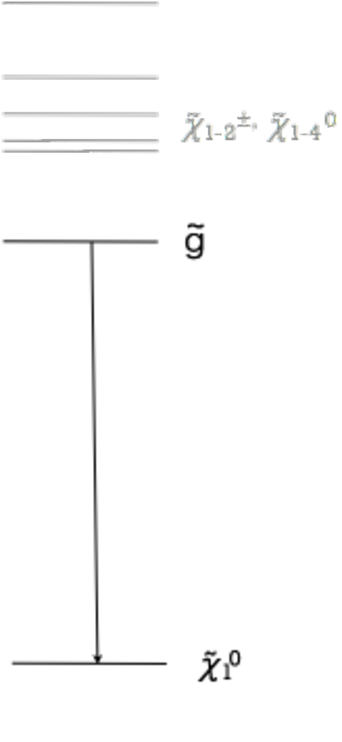
\includegraphics[width=0.21\textwidth]{figures/Introduction/massConfig_direct.pdf}}
    \subfigure[]{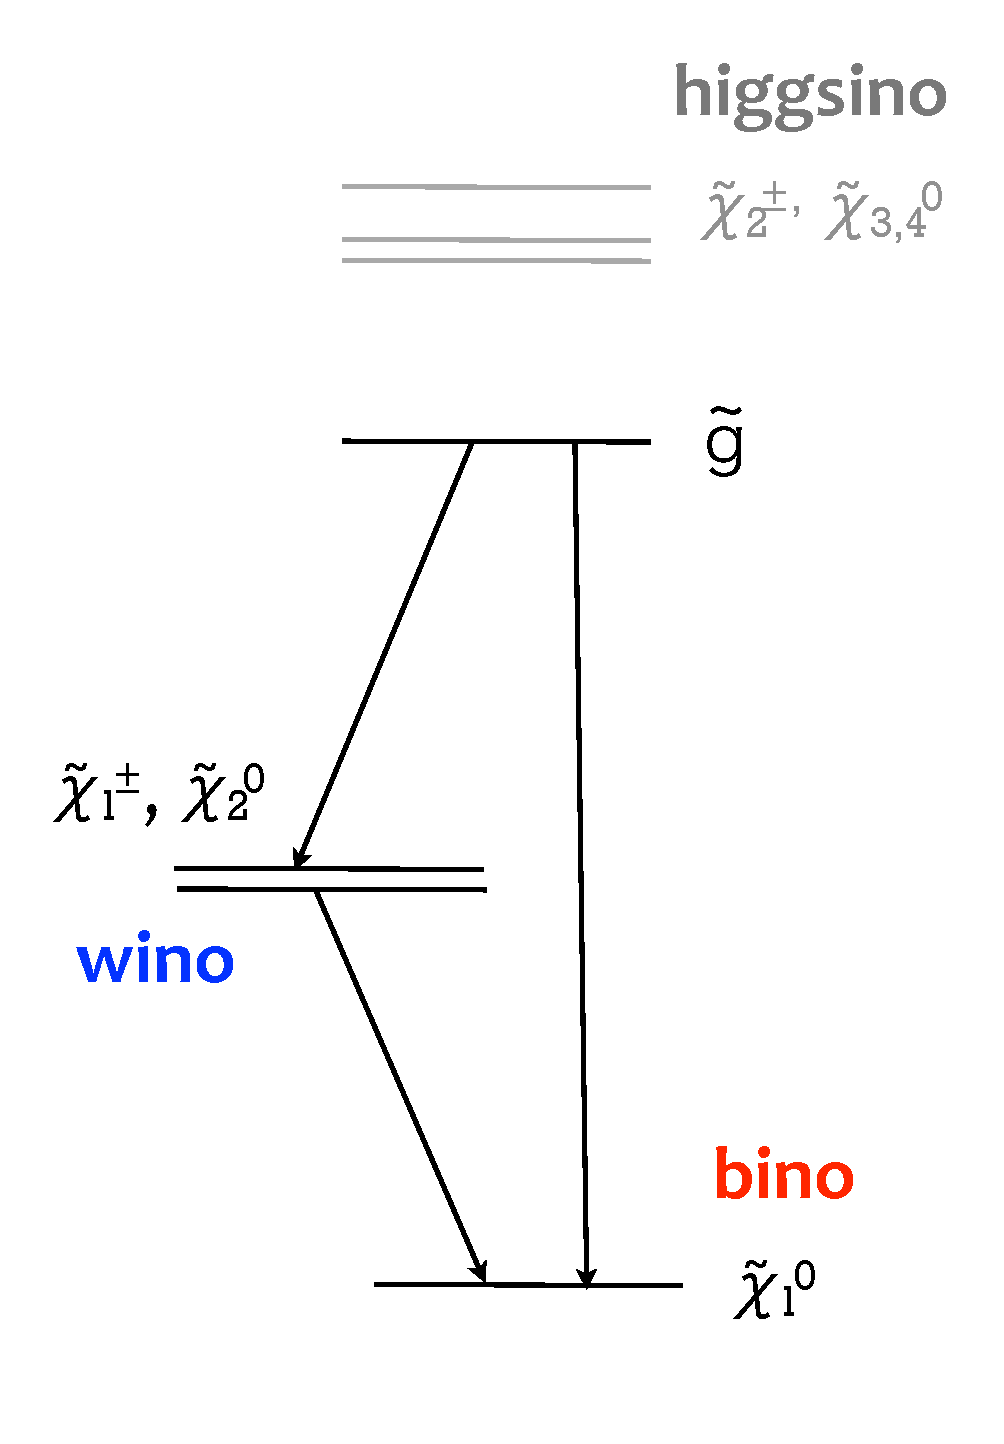
\includegraphics[width=0.38\textwidth]{figures/Introduction/massConfig_no_higgsino.pdf}}
    \subfigure[]{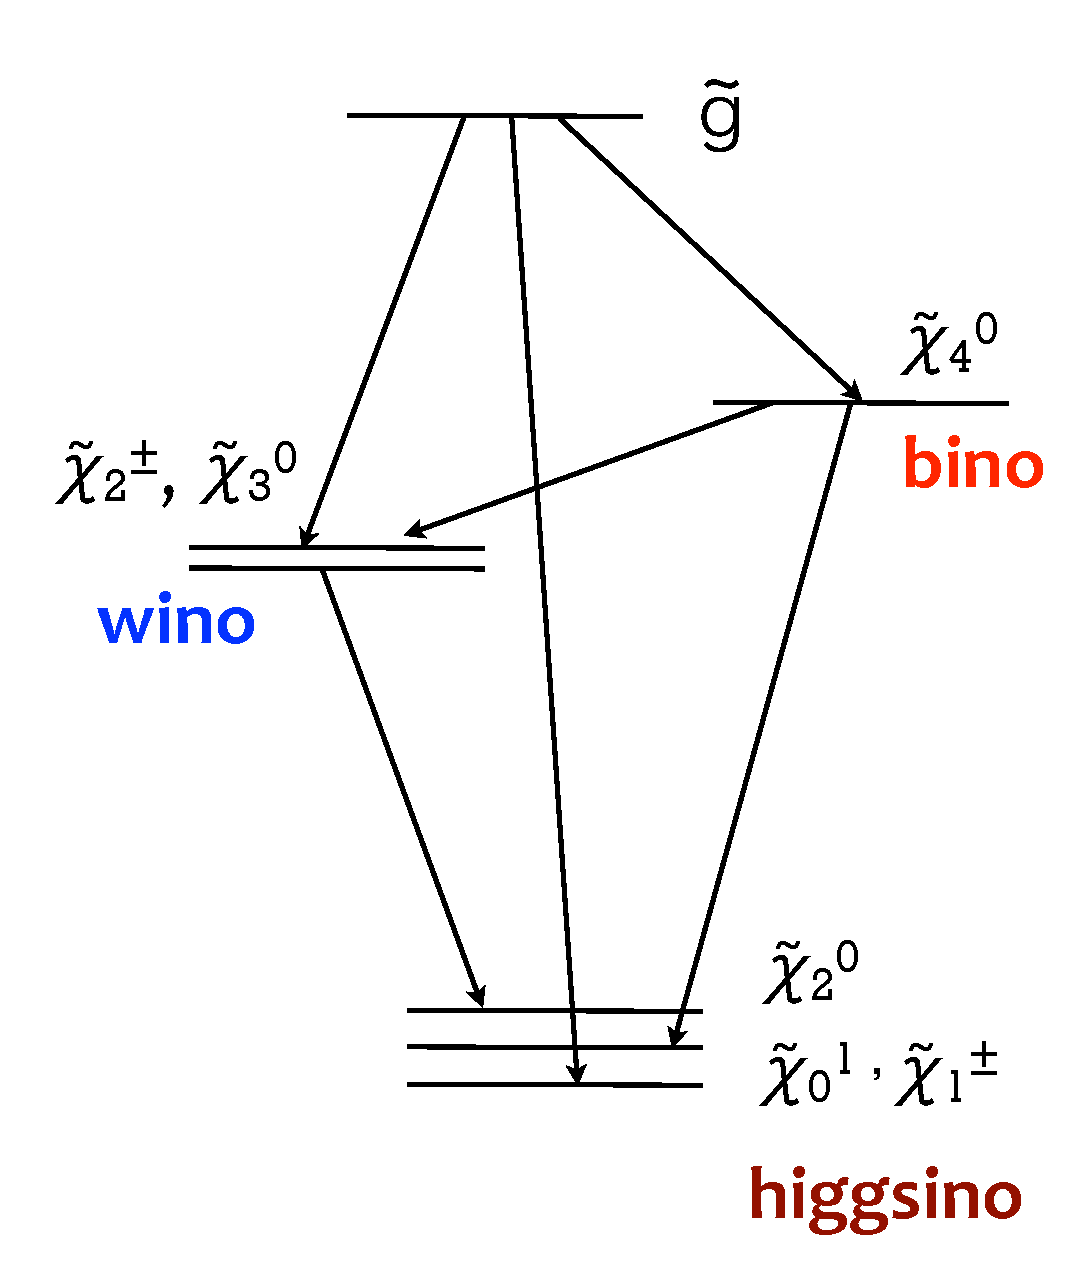
\includegraphics[width=0.38\textwidth]{figures/Introduction/massConfig_with_higgsino.pdf}}
    \caption{ 
Possible gluino decay paths are illustrated for mass spectra where
(a) all the EW gauginos are heavier than gluino ($100\%$ direct decay of gluino),
(b) higgsinos are heavier than gluino while the other EW gauginos are lighter (mixture of direct decay and 1-step decays),
(c) all the EW gauginos are below gluino mass (mixture of direct decay, and numerous 1-step and 2-step decays),
are illustrated.
The hieararchy between wino and bino in (b), or between all the EW gauginos in (c) are also allowed.
\label{fig::Introduction::signal_massConfig} }
\end{figure}
%%%%%%%%%%

As for the scenario in Fig. \ref{fig::Introduction::signal_massConfig}, a numerious MSSM parameters scans demonstrate that the probability of 2-stes decays are generally much lower than that of direct or 1-step decays, except for some of the cases where each of the intermideate masses are aligned with relatively equal distance 
%(See Appendix)
. Therefore, in the analysis, we confine our scope within direct and 1-step decay of gluino. \\

The acceptance dependence between ligh quark flavors ($u,d,s,c$) are also small, therefore can be merged i.e. a simplified model where gluino decays with equal rate between $u,d,s,c$ is considered. \\

For seb-sequent gaugino decays, charginos are assumed always decays into on-shell or off-shell $W$-boson, while two options for neutralinos decays via $Z/h$ are considred. The decays into slepton is ignored here, majorly for convenience sake of restricting the number of final states, however with a few justifications; under a general unification regime, slepton masses are order of squark masses which are considered to be $>3\tev$; when respecting the observed DM relic abundance, the mass splitting between NLSP and LSP becomes naturally small (typically $<50\gev$). Decays via sleptons requires sleptons masses in between NLSP and LSP, which is unlikely to happen. \\

With all the scrutinization, the targeted gluino decay chains are reduced into Tab. \ref{tab::Introduction::gluinoDecay2}.
Corresponding Feymann diagrams are shown in Fig. \ref{fig::Introduction::gluinoDecay_summary}. 
\tab{c|l}{
\hline
Direct decay (3) & $\tg \ra (q\bar{q},q\bar{q},q\bar{q}) \tilde{\chi}_{1}^{0}$  \\
\hline
\hline
1-step decay (8) & $\tg \ra (q\bar{q}', t\bar{b}(b\bar{t})) \,\,\, \tilde{\chi}_{1}^\mp, \,\,\,\,\,\,\, \tilde{\chi}_{1}^- \ra W^\mp \tilde{\chi}_{1}^{0} $ \\
                 & $\tg \ra (q\bar{q}, b\bar{b},t\bar{t}) \,\,\,  \tilde{\chi}_{2}^{0}, \,\,\,\,\, \tilde{\chi}_{2}^{0} \ra Z\tilde{\chi}_{1}^{0})$ \\
                 & $\tg \ra (q\bar{q}, b\bar{b},t\bar{t})  \,\,\, \tilde{\chi}_{2}^{0}, \,\,\,\,\, \tilde{\chi}_{2}^{0} \ra h\tilde{\chi}_{1}^{0})$ \\ 
\hline
}
{Summary of targeted gluino decay chains. The number in the pharenthese indicates the numbers of chains in the categoty.}
{tab::Introduction::gluinoDecay2}


\fig[150]{Samples/signalModels/gluinoDecay_summary.pdf}
{Target gluino decay chains.}
{fig::Introduction::gluinoDecay_summary}


The full decay chains of pair produced gluinos become increasingly complicated: 11 symmetric decays (two gluinos experience the same decay chains), 55 symmetric decays (two gluinos experience different decay chains).
In total, 66 decay chains are identified as the targets. \\


\subsubsection{Target Signal Models for 1-lepton Final State}
In LHC, analyzes are conventionally divided based on number of hard leptons in the final state, since eiter signal kinematics and the background strategy are drastically different. In gluino decays, ignoring the decays into sleptons, leptons are always generated via decays of W/Z/H boson. Therefore, giving their small leptonical branching ratio, 0-lepton or 1-lepton final state are the most promissing channel for inclusive search, while 2/3-leptons final states are more specialized in specific types of scenarios such as long-chain multi-step gluino decays where more W/Z/H bosons are involved. \\

This thesis focus on the final state with exactly one lepton. 
Therefore decay chains with marginal branching ratio into final state with exactly 1-lepton will be excluded from the targets. 
The full list of the target decay chains in the thesis (referred as ``benchmark model'') are shonw in Tab. \ref{tab::Introduction::modelsBV} - Tab. \ref{tab::Introduction::models3B}, with the naming convention for each decay chain defined as Eq. (\ref{eq::gridNameConvention}). They are further categorized based on the number of expected b-quarks in the final state, as the signal regions will be segmented based on the numberof b-tagged jets. The reference models for each b-categories are respectively chosen as \textbf{QQC1QQC1},\textbf{QQC1BTC1} and \textbf{TTN1TTN1} for BV, BT and 3B (Fig. \ref{fig:Introduction::refModels}), which will be used as the reference in designing signal regions and other various studies. The Feynman deagrams for the reference models are illustrated in Fig. \ref{fig:Introduction::refModels}.

%Although the 0-lepton final state often is more advantageous in terms of coverage of models and signal acceptance, 1-lepton addresses some unique merits over the 0-lepton channel as following:
%- 0Lよりclean. QCDとかnon-collisionみたいな変なBGの心配をしなくていい
%- 2Lよりはsignalが多い. 2LをCRにできる.  (0Lで1LをCRとすると結構contamiが無視できない?)  あとCRがpure
%- 0Lとのcincidenceを取ることでSUSYとのconsistencyについて議論できる

% compressedとかだとそこに書いてあるよりmultiplicity減るっていうことにも一応言及

\begin{align}
  \mbox{Model name} & := aaXXbbYY  \nn \\
  aa,bb & = \mbox{``QQ'',``BB'',``TT'',``BT''}  \nn \\
  XX,YY & = \mbox{``N1'',``C1'',``N2Z'',``N2H''} 
%  \label{eq::gridNameConvention}
\end{align}

%%%%%%%%%%%%%%%%%%%%%%%


\tab{c c c c c c}{
  \hline
  \textbf{1-step decay}  & $n_{\mathrm{J}}$ &  $n_{\mathrm{B}}$ & Br(1L)/Br(0L) & Br(1L)/Br(2L)  & det sim.?  \\ \hline
  \hline
  QQN1QQC1 & 5.5 & 0.0 & 0.33 & - & \\ \hline
  \textcolor{red}{\textbf{QQC1QQC1}} & 7.0 & 0.0 & 0.67 & 6 & \checkmark   \\ \hline
  QQC1QQN2Z & 7.3 & 0.3 & 0.35 & 3.86 & \checkmark   \\ \hline
  \hline
}
{Target models with no b-jets at tree level (BV models). The average jet multiplicity ($n_{\mathrm{J}}$) and b-jet multiplicity ($n_{\mathrm{B}}$) are calculated based on number of quarks and b-quarks appearing in the final state. The PDG values \cite{PDG2016} are referred for branching ratio of top, W/Z/h bosons. $``\checkmark''$ specifies the models with the final result derived using the samples with the fast detector simulation (ATLFast 2 ~\cite{atlfast}), while the others are with emulated truth samples.}
{tab::Introduction::modelsBV}



\tab{c c c c c c}{
  \hline
  \textbf{Direct decay}  & $n_{\mathrm{J}}$ &  $n_{\mathrm{B}}$ & Br(1L)/Br(0L) & Br(1L)/Br(2L)  & det sim.?  \\ \hline
  \hline
  QQN1TTN1 & 7.0 & 2.0 & 0.67 & 6 & \\ \hline
  \hline
  \textbf{1-step decay}  & $n_{\mathrm{J}}$ &  $n_{\mathrm{B}}$ & Br(1L)/Br(0L) & Br(1L)/Br(2L)  & det sim.?  \\ \hline
  \hline
  QQC1QQN2H & 7.4 & 1.1 & 0.46 & 7.07 & \checkmark   \\ \hline
  QQN1BTC1 & 7.0 & 2.0 & 0.67 & 6 & \\ \hline
  QQN1TTN2Z & 8.8 & 2.3 & 0.68 & 3.30 & \\ \hline
  \textcolor{red}{\textbf{QQC1BTC1}} & 8.5 & 2.0 & 1.0 & 3 & \checkmark   \\ \hline
  QQC1BBN2Z & 7.3 & 2.3 & 0.35 & 3.86 & \\ \hline
  QQC1TTN2Z & 10.3 & 2.3 & 1.02 & 2.34 & \\ \hline
  QQN2ZTTN2Z & 10.7 & 2.6 & 0.7 & 2.31 & \\ \hline
  BBN1QQC1 & 5.5 & 2.0 & 0.33 & - & \\ \hline
  BTC1QQN2Z & 8.8 & 2.3 & 0.68 & 3.30 & \\ \hline
  TTN1QQC1 & 8.5 & 2.0 & 1.0 & 3 & \\ \hline
  TTN1QQN2Z & 8.8 & 2.3 & 0.68 & 3.30 & \\ \hline
  \hline
}
{Target models with 1 or 2 b-jets at tree level (BT models). 
Definition of $n_{\mathrm{B,J}}$, branching and $``\checkmark''$ are the same as Table \ref{tab::Introduction::modelsBV}.}
{tab::Introduction::modelsBT}



\tab{c c c c c c}{
  \hline
  \textbf{Direct decay}  & $n_{\mathrm{J}}$ &  $n_{\mathrm{B}}$ & Br(1L)/Br(0L) & Br(1L)/Br(2L)  & det sim.?  \\ \hline
  \hline
  BBN1TTN1 & 7.0 & 4.0 & 0.67 & 6 & \\ \hline
  \textcolor{red}{\textbf{TTN1TTN1}} & 10 & 3.9 & 1.33 & 2 & \checkmark   \\ \hline
  \hline
  \textbf{1-step decay}  & $n_{\mathrm{J}}$ &  $n_{\mathrm{B}}$ & Br(1L)/Br(0L) & Br(1L)/Br(2L)  & det sim.?  \\ \hline
  \hline
  QQN1TTN2H & 8.9 & 3.1 & 0.79 & 3.64 & \\ \hline
  QQC1BBN2H & 7.4 & 3.1 & 0.46 & 7.07 & \\ \hline
  QQC1TTN2H & 10.4 & 3.1 & 1.12 & 2.34 & \\ \hline
  QQN2ZTTN2H & 10.8 & 3.4 & 0.8 & 2.56 & \\ \hline
  QQN2HTTN2H & 10.8 & 4.3 & 0.91 & 2.70 & \\ \hline
  BBN1BTC1 & 7.0 & 4.0 & 0.67 & 6 & \\ \hline
  BBN1TTN2Z & 8.8 & 4.3 & 0.68 & 3.30 & \\ \hline
  BBN1TTN2H & 8.9 & 5.1 & 0.79 & 3.64 & \\ \hline
  BBN2ZTTN2Z & 10.7 & 4.6 & 0.7 & 2.31 & \\ \hline
  BBN2ZTTN2H & 10.8 & 5.4 & 0.8 & 2.56 & \\ \hline
  BBN2HTTN2H & 10.8 & 6.3 & 0.91 & 2.70 & \\ \hline
  BTC1QQN2H & 8.9 & 3.1 & 0.79 & 3.64 & \\ \hline
  BTC1BTC1 & 10 & 4.0 & 1.33 & 2 & \\ \hline
  BTC1BBN2Z & 8.8 & 4.3 & 0.68 & 3.30 & \\ \hline
  BTC1BBN2H & 8.9 & 5.1 & 0.79 & 3.64 & \\ \hline
  BTC1TTN2Z & 11.8 & 4.3 & 1.35 & 1.75 & \\ \hline
  BTC1TTN2H & 11.9 & 5.1 & 1.46 & 1.70 & \\ \hline
  TTN1QQN2H & 8.9 & 3.1 & 0.79 & 3.64 & \\ \hline
  TTN1BTC1 & 10 & 4.0 & 1.33 & 2 & \\ \hline
  TTN1BBN2Z & 8.8 & 4.3 & 0.68 & 3.30 & \\ \hline
  TTN1BBN2H & 8.9 & 5.1 & 0.79 & 3.64 & \\ \hline
  TTN1TTN2Z & 11.8 & 4.2 & 1.35 & 1.75 & \\ \hline
  TTN1TTN2H & 11.9 & 5.1 & 1.46 & 1.70 & \\ \hline
  TTN2ZQQN2H & 10.8 & 3.4 & 0.8 & 2.56 & \\ \hline        
  TTN2ZBBN2H & 10.8 & 5.4 & 0.8 & 2.56 & \\ \hline
  TTN2ZTTN2Z & 13.7 & 4.5 & 1.36 & 1.55 & \\ \hline
  TTN2ZTTN2H & 13.8 & 5.4 & 1.47 & 1.53 & \\ \hline
  TTN2HTTN2H & 13.8 & 6.2 & 1.58 & 1.49 & \\ \hline
  \hline
}
{Target models with 3 or more b-jets at tree level (3B models).
Definition of $n_{\mathrm{B,J}}$, branching and $``\checkmark''$ are the same as Table \ref{tab::Introduction::modelsBV} and \ref{tab::Introduction::modelsBT}.}
{tab::Introduction::models3B}

%%%%%%%%%%%%%%%%%%%%


\begin{figure}[h]
  \centering
    \subfigure[]{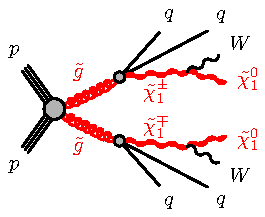
\includegraphics[width=0.32\textwidth]{figures/diagrams/GG_QQC1QQC1.pdf}}
    \subfigure[]{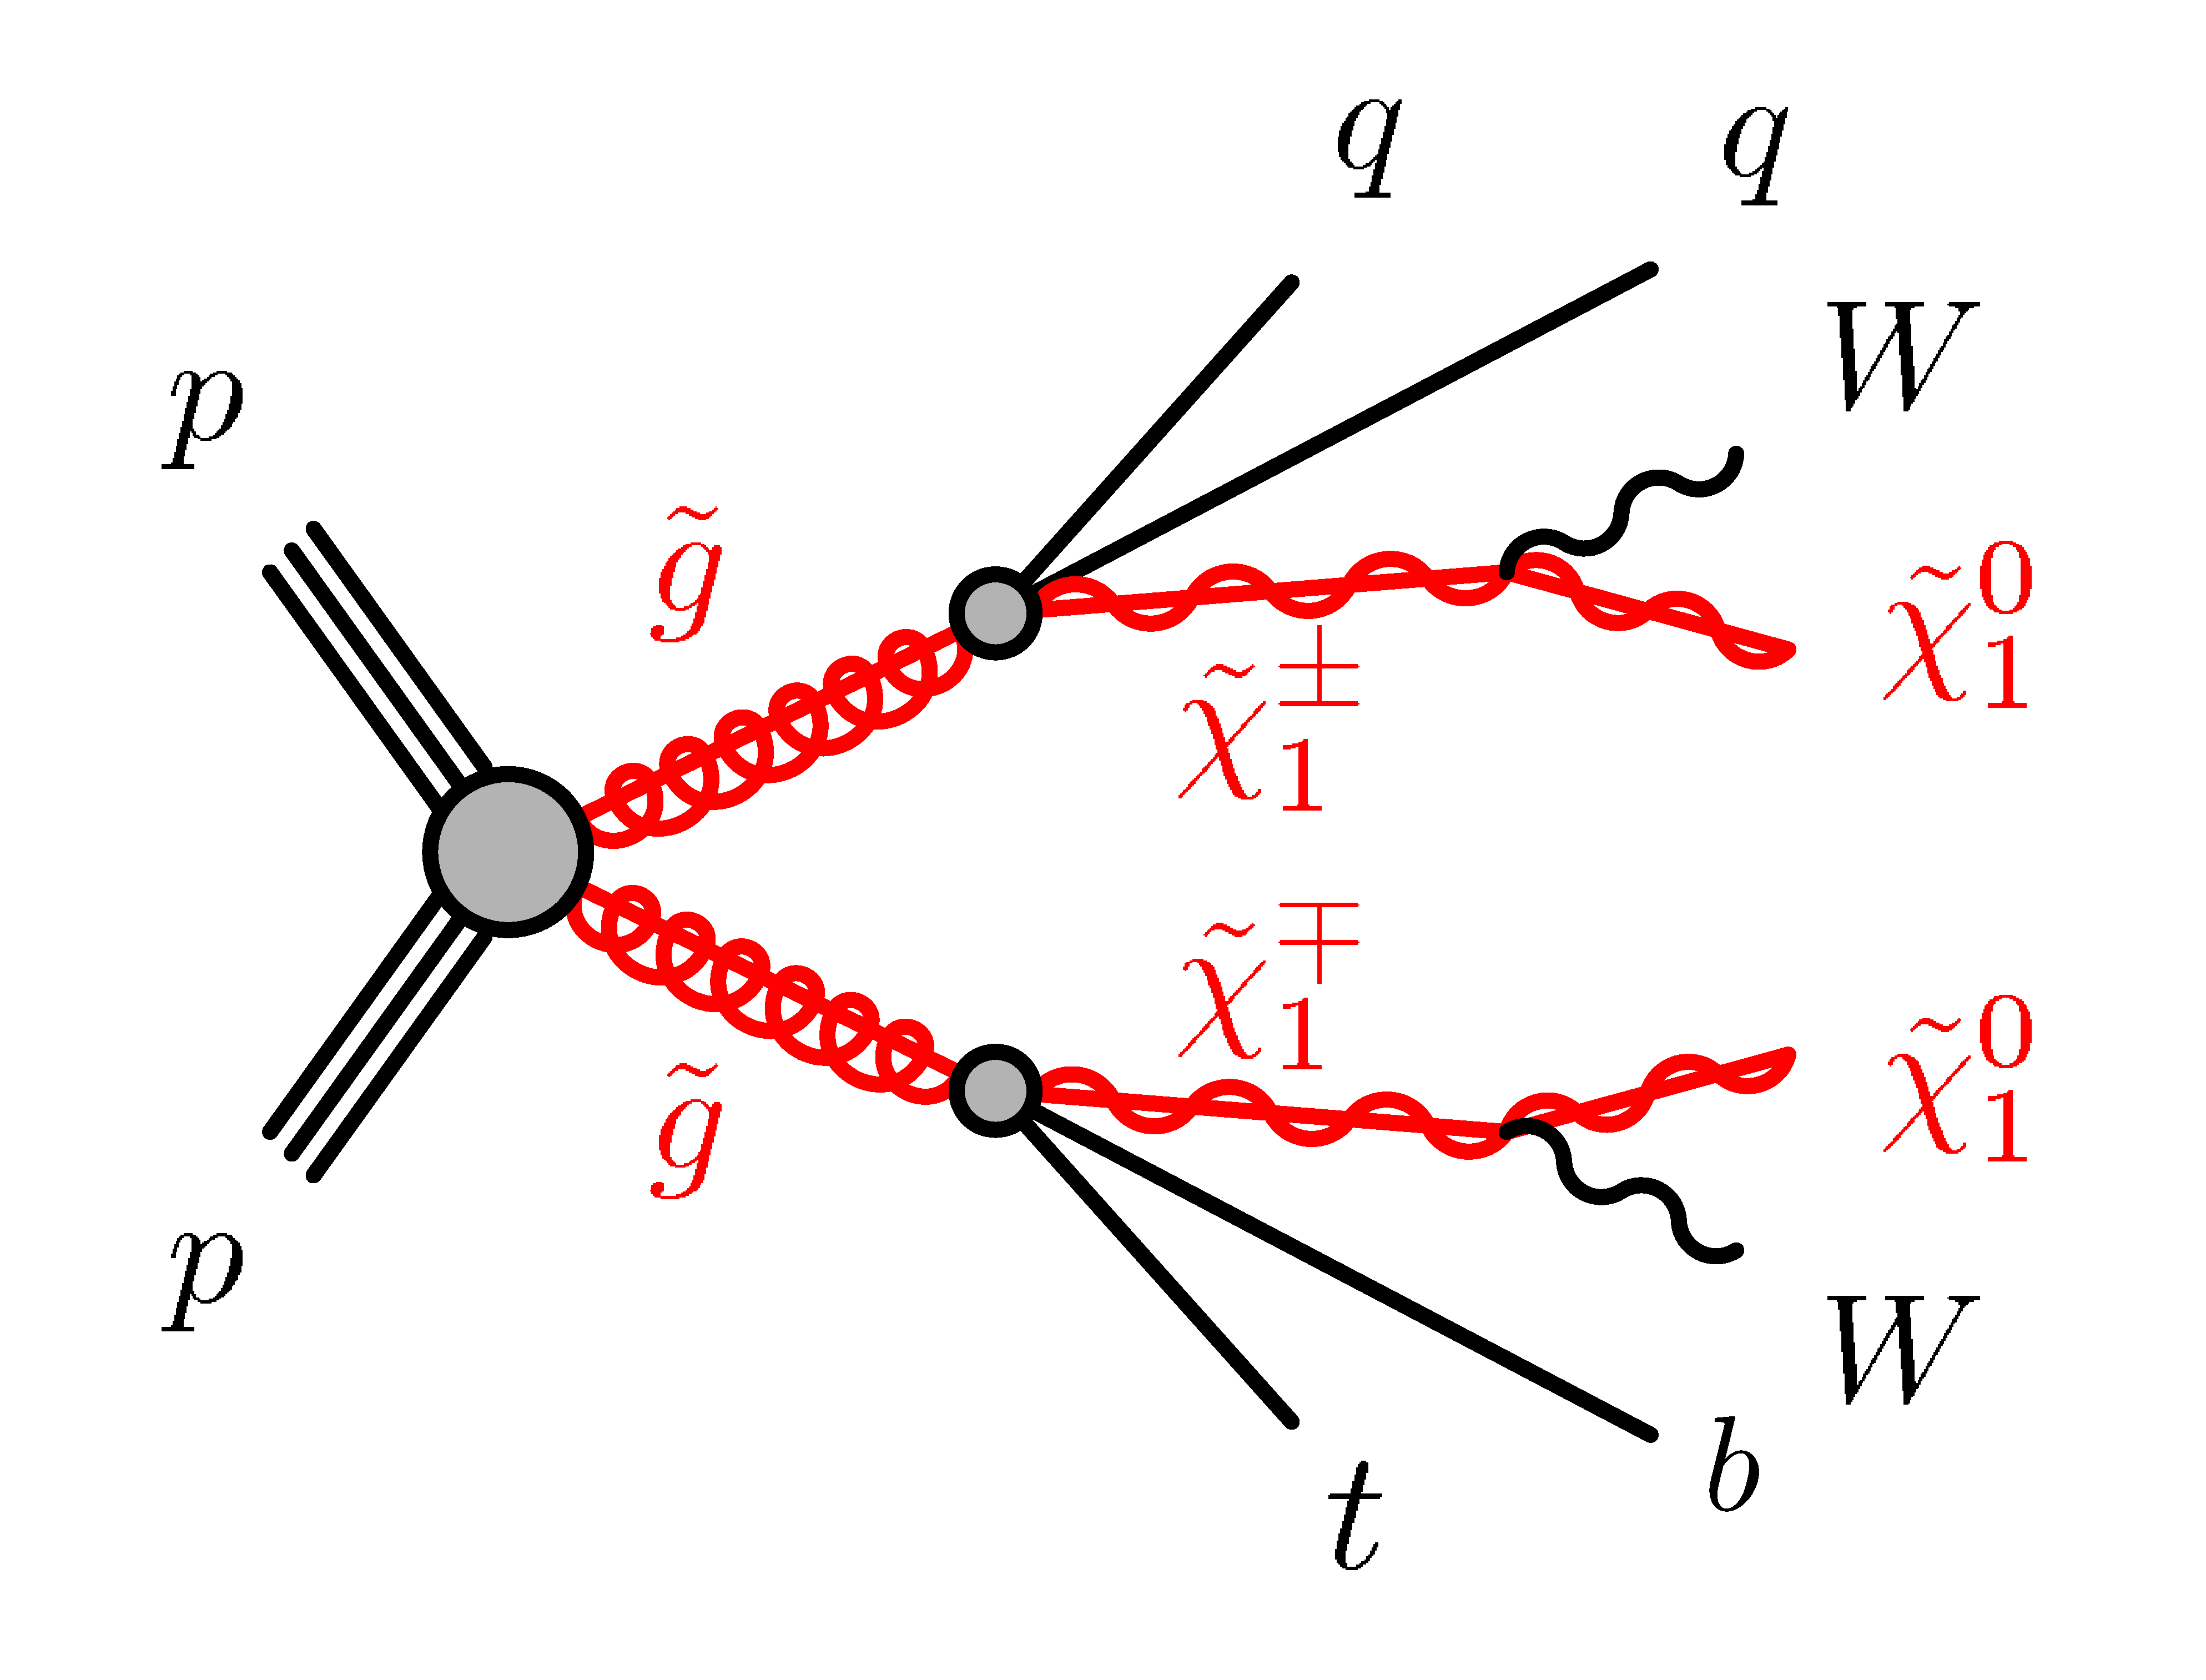
\includegraphics[width=0.32\textwidth]{figures/diagrams/GG_QQC1BTC1.pdf}}
    \subfigure[]{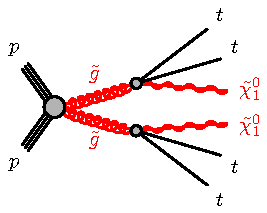
\includegraphics[width=0.32\textwidth]{figures/diagrams/GG_TTN1TTN1.pdf}}
    \caption{ Feymann diagrams for the Benchmark models (a) QQC1QQC1 (b) QQC1BTC1 (c) TTN1TTN1. }
    \label{fig:Introduction::refModels}
\end{figure}



\subsection{Structure of the thesis}
The rest of the sections will proceed as follow: 
The LHC and the ATLAS detector is firstly overviewed in Sec. \ref{sec::Detector}, 
to have idea of typical environment that LHC provides and 
the precision the ATLAS detectors system offers ; 
Sec. \ref{sec::objDef} follows with describing the off-line algorithms of reconstructions and identifications for particles or jets; 
The detail of simulation used in analysis is given in Sec. \ref{sec::Samples}; 
The description of the analysis starts with Sec. \ref{sec::SRdefinition} in which the preselection and signal regions are designed. Sec. \ref{sec::BGestimaiton} is then involve comprehensive discussion on the background estimation, the most important part in the analysis;
Uncertainties associated with background estimation and signal modeling is overviewed in Sec. \ref{sec::Uncertainties}
; finally the unblinded result and resultant limits are shown in Sec. \ref{sec::Result}; 
with brief conclusion remarks in Sec. \ref{sec::Conclusion}.


